\chapter{Síntesis de software para GNC embebido}
\label{ch:especifico2}

Como se pudo observar en el capítulo \ref{ch:especifico1}, se realizó la selección de la tarjeta de desarrollo Zedboard, además de esto uno de los requerimientos que se tomó en cuenta fue la compatibilidad de esta con el flujo de trabajo de Yocto Project.

\begin{figure}[h!]
    \centering
    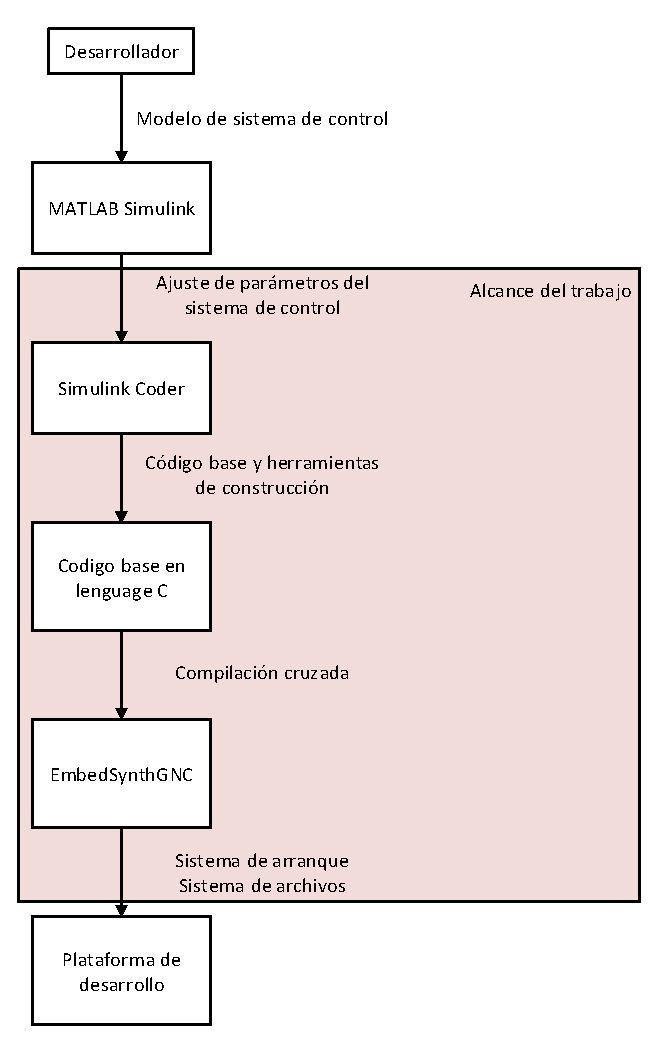
\includegraphics[width=0.48\textwidth]{fig/especifico_2/Diagrama general del proyecto.pdf}
    \caption{Diagrama general del flujo de trabajo propuesto}
    \label{fig:diagrama_flujo_trabajo}
\end{figure}

En este capítulo se pretende establecer los flujos de trabajo para el prototipado de algoritmos de control, orientación y navegación para aplicaciones espaciales. Esto mediante la implementación de un caso de estudio básico. Como se puede observar en la Figura \ref{fig:diagrama_flujo_trabajo}, primeramente el desarrollador toma un modelo de sistema de control, el cual debe implementar en MATLAB Simulink por medio de los bloques del sistema. 

Seguido de esto se realiza un ajuste de parámetros con el objetivo que el mismo opere dentro de las condiciones esperadas, una vez ajustado el sistema, se debe de ingresar el modelo al flujo de trabajo de Simulink Coder, el cual nos dará como salida el código base y las herramientas de construcción requeridas para poder compilar el archivo ejecutable, cabe destacar que la compilación a realizar es cruzada, esta nos permite compilar los archivos en un sistema distinto al objetivo. 

Finalmente se debe de ingresar el archivo binario generado al flujo de trabajo de EmbedSynthGNC, el cual, se encargara de dar como salida un sistema de archivos de arranque y el sistema de directorios listos para implementar en la plataforma de desarrollo.


\section{Creación de los entornos de desarrollo}

En esta sección se describen los pasos necesarios para la creación de los entornos de desarrollo utilizados en este proyecto. En el mismo se incluye la información del hardware y software utilizado, además de las versiones de los sistemas para cada una de las implementaciones. Cabe destacar que el computador anfitrión en el cual se implementan estos entornos de desarrollo tiene las siguientes características:

\begin{itemize}
    \item Procesador Intel i9 - 13900k 
    \item Almacenamiento 1 TB
    \item Memoria 16 GB
    \item Video Nvidia RTX4060Ti
\end{itemize}

\subsection{MATLAB}\label{subsec:generacion_entorno_matlab}

Para el entorno de MATLAB se utiliza como sistema operativo Windows 11, en su versión de 64 bits, se destina a este sistema operativo un espacio en disco de 500 GB, en el cual se instalen los programas requeridos para la generación de contenido y el análisis de datos. La versión utilizada es MATLAB 2024b por medio de una licencia de prueba de la versión full, la cual nos permitirá generar y probar el contenido necesario para los casos de uso a tratar. Por otro lado, para el análisis y procesamiento de datos se utiliza Python 3.12.3.

\begin{figure}[h!]
    \centering
    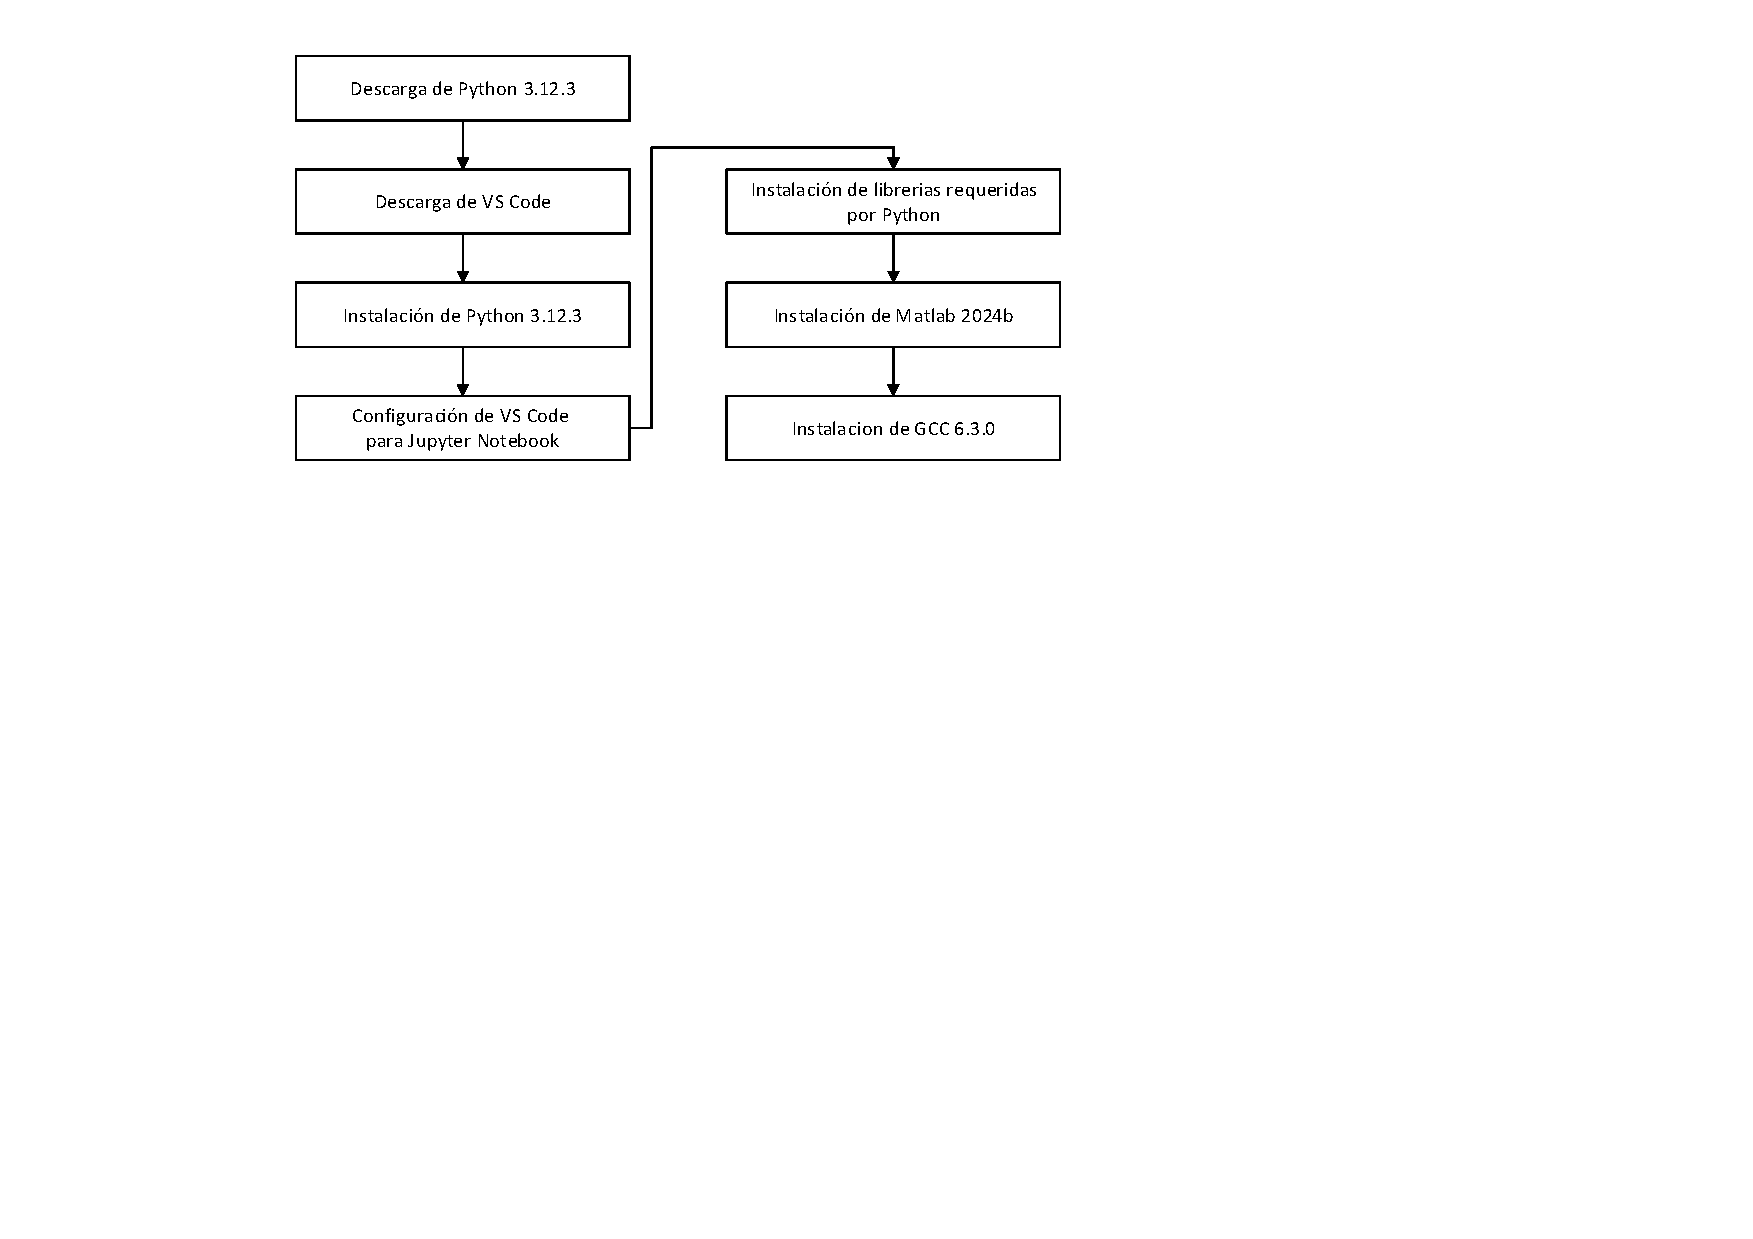
\includegraphics[width=0.3\textwidth]{fig/especifico_2/Entorno_windows}
    \caption{Diagrama para generar el entorno de MATLAB}
    \label{fig:diagrama_entorno_matlab}
\end{figure}

Como se muestra en la Figura \ref{fig:diagrama_entorno_matlab}, para la generación de este entorno de trabajo primeramente se deberá de realizar la instalación de Python 3.12.3 y seguido de esto la instalación de MATLAB con las herramientas requeridas. Finalmente se debe de instalar GCC en su versión 6.3.0.

Primeramente se debe de realizar la descarga de Visual Studio desde \href{https://code.visualstudio.com/sha/download?build=stable&os=win32-x64-user}{este enlace}, esto con el fin de poder hacer uso de Jupyter Notebook para el análisis de datos, además de esto se debe de descargar Python en su versión 3.12.3 desde esta \href{https://www.python.org/ftp/python/3.12.3/python-3.12.3-amd64.exe}{dirección}. 


\begin{figure}[h!]
    \centering
    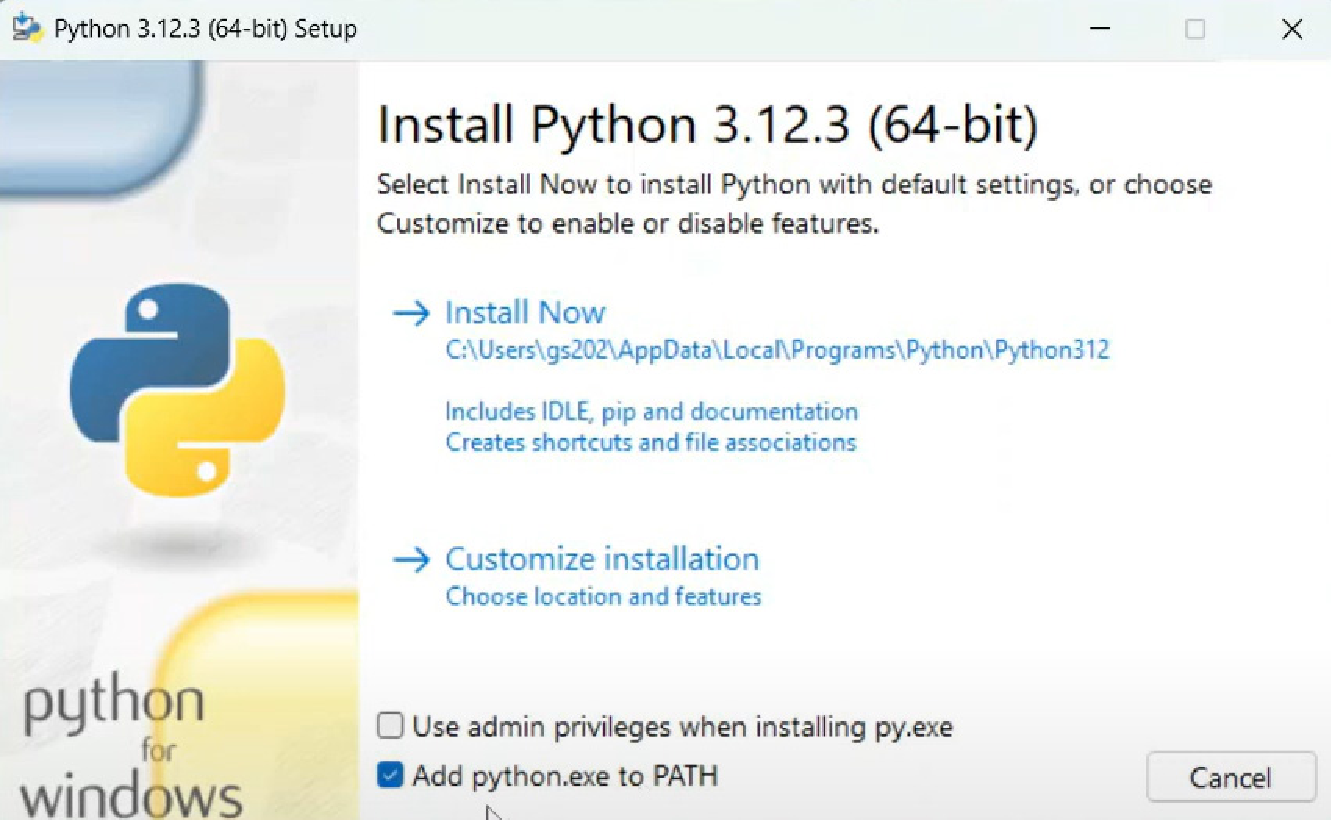
\includegraphics[width=0.45\textwidth]{fig/especifico_2/Ambiente_matlab/instalacion_python.pdf}
    \caption{Menú de instalación de Python}
    \label{fig:menu_python}
\end{figure}


\begin{figure}[h!]
    \centering
    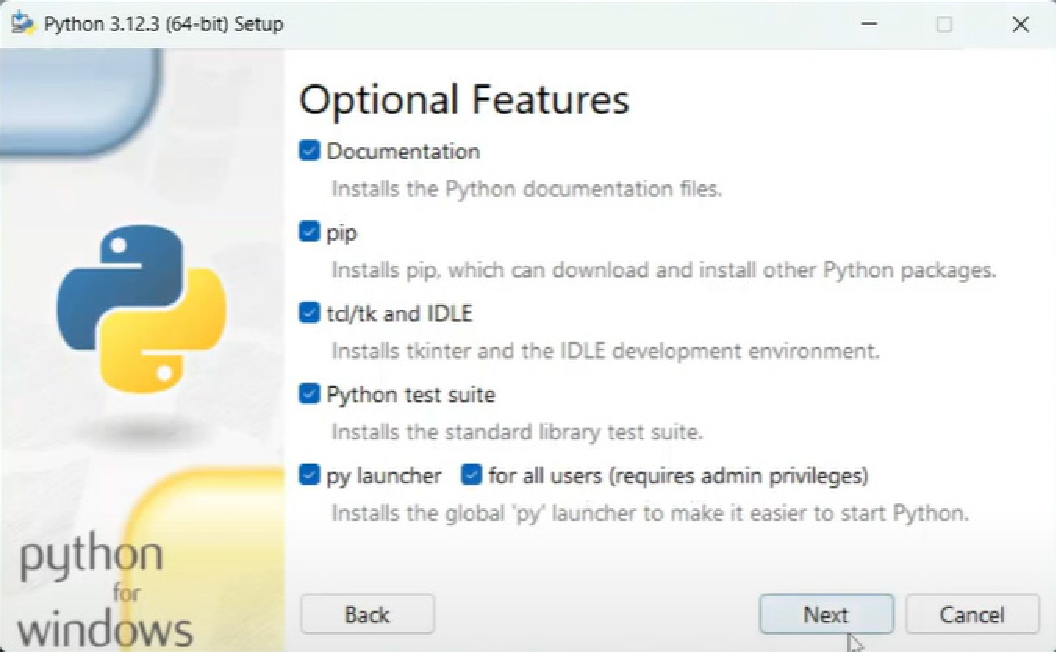
\includegraphics[width=0.45\textwidth]{fig/especifico_2/Ambiente_matlab/opciones_adicionales_python.pdf}
    \caption{Menú de instalación de Python}
    \label{fig:menu_python_adicionales}
\end{figure}

Una vez descargados estos programas se debe de realizar la instalación de los mismos, primeramente se debe de instalar Python, el cual como se observó en la Figura \ref{fig:menu_python} se debe de seleccionar la opción para agregar Python al directorio PATH, esto con el fin de poder instalar los entornos y librerías requeridas. Seguido de esto se debe de seleccionar la opción de instalación personalizada (Customize installation) con el fin de poder agregar las características que se mostraron en la Figura \ref{fig:menu_python_adicionales}. 

\begin{figure}[h!]
    \centering
    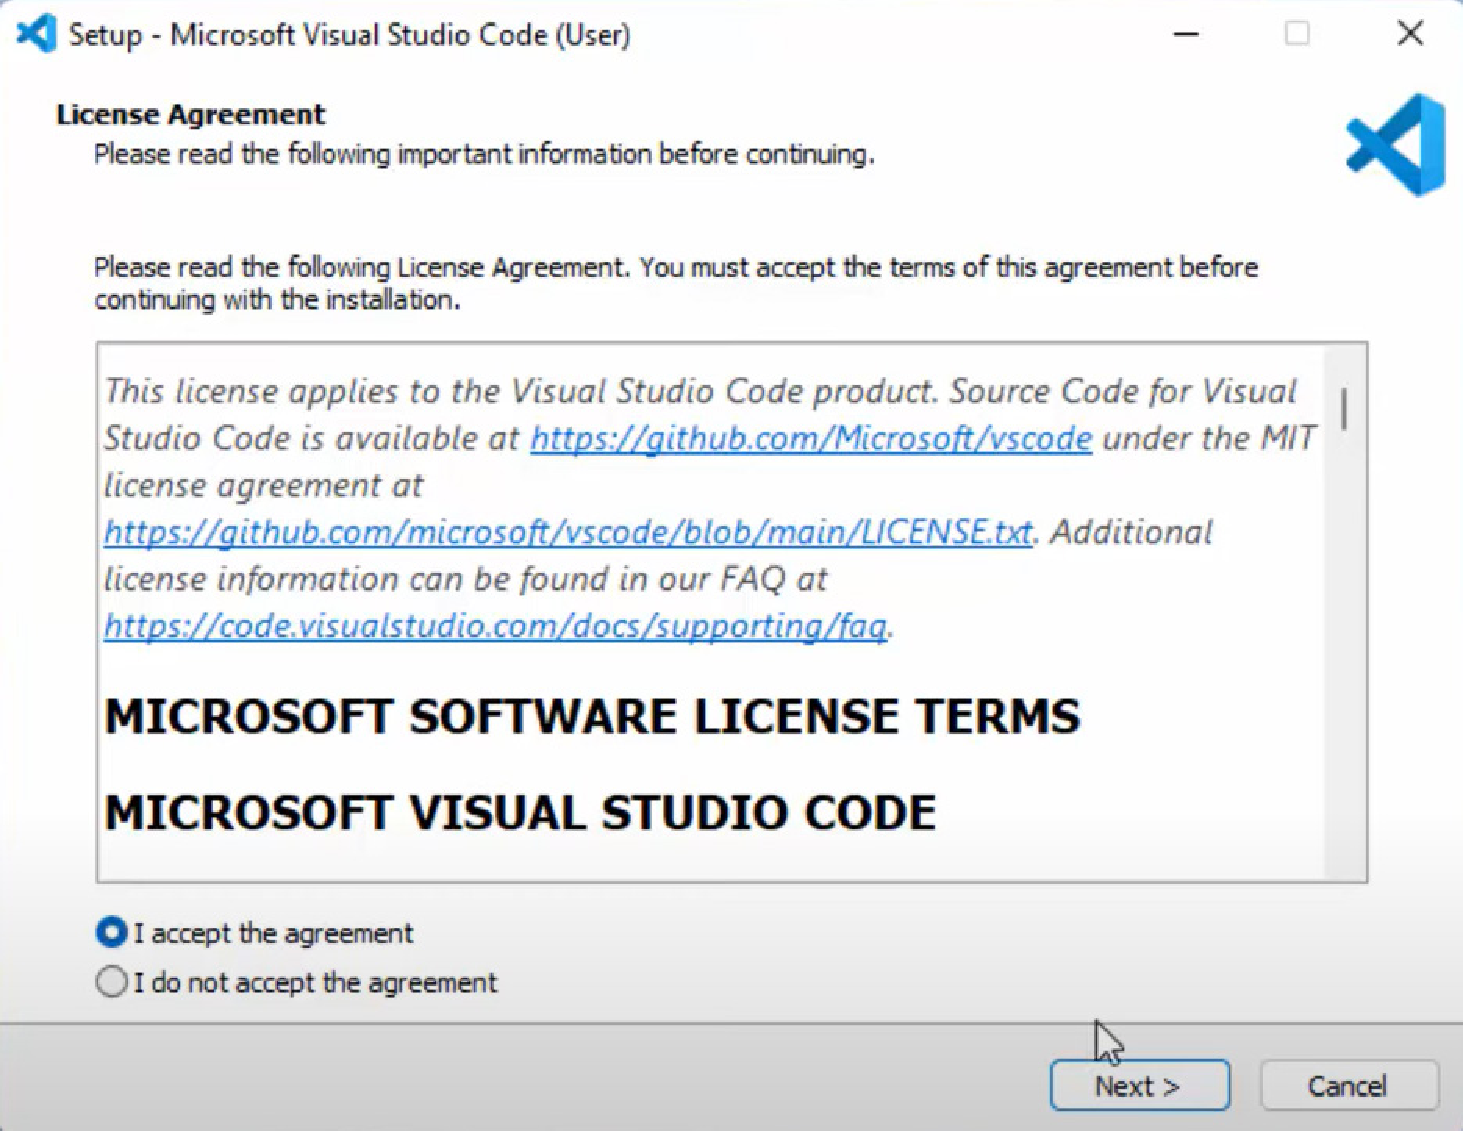
\includegraphics[width=0.45\textwidth]{fig/especifico_2/Ambiente_matlab/instalacion_vs_code.pdf}
    \caption{Menú de instalación de VS Code}
    \label{fig:menu_vscode}
\end{figure}


\begin{figure}[h!]
    \centering
    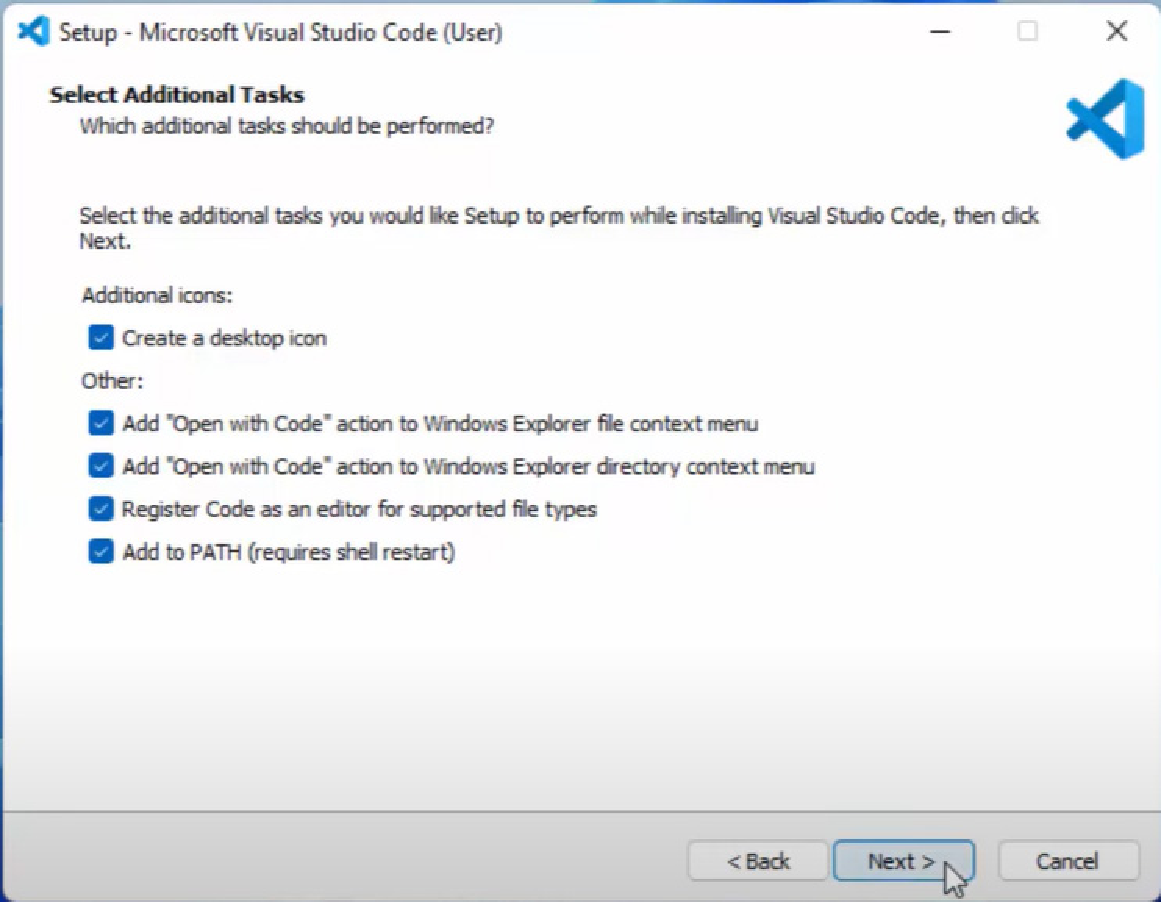
\includegraphics[width=0.45\textwidth]{fig/especifico_2/Ambiente_matlab/opciones_adicionales_vs_code.pdf}
    \caption{Menú de instalación de VS Code}
    \label{fig:menu_vscode_adicionales}
\end{figure}

Una vez concluida la instalación de Python se debe proseguir con VS Code, el cual como se pudo observar en la Figura \ref{fig:menu_vscode}, se deben de aceptar los términos y condiciones del programa y en el siguiente menú se deben seleccionar las opciones marcadas en la Figura \ref{fig:menu_vscode_adicionales}.

Finalmente se debe de realizar la descarga de MATLAB la cual se puede conseguir por medio de \href{https://matlab.mathworks.com/}{este enlace}, se debe de generar una cuenta y descargar la versión de prueba que tiene una durabilidad de 30 días, o bien si se cuenta con la licencia del producto no es necesario recurrir a esta. Dentro de la instalación es importante mencionar que se podrán solicitar todas las herramientas dentro del periodo de prueba, pero las que son fundamentales para el desarrollo del mismo son las siguientes:

\begin{itemize}
    \item MATLAB Simulink
    \item MATLAB Coder
\end{itemize}

Además, se instala la herramienta GCC en su versión 6.3.0, el cual es el compilador de código C, este se utilizara para compilar el código y probar que el mismo funcione de la forma esperada; cabe destacar, que este no es el compilador cruzado, este compilador nos genera un archivo binario el cual podremos probar en el sistema Windows, esto con el fin de poder realizar correcciones más eficientes al sistema de control en caso de ser requerido.

\subsection{Contenedores}\label{sec:entorno_en_contenedores}

En la elaboración del proyecto se decanta por el uso de contenedores, ya que como se mencionó en \ref{sec:containers}, estos permiten encapsular todas las dependencias y configuraciones necesarias para ejecutar una aplicación. Esto asegura que la misma aplicación funcione de manera consistente en diferentes entornos, ya sea durante el desarrollo, en pruebas o en producción. 

Cada contenedor opera de forma independiente, lo que permite ejecutar múltiples aplicaciones en el mismo sistema sin interferencias. Este aislamiento reduce significativamente el riesgo de conflictos entre diferentes versiones de software y dependencias, lo que se traduce en un entorno más estable y predecible. Los contenedores se elaboran en el computador anfitrión en un sistema operativo Linux en su versión 22.04 LTS.

\subsubsection{Comandos utilizados para la creación y gestión de contenedores}\label{subsec:manejo_de_contenedores}


\begin{lstlisting}[language=bash, caption={Instalacion de docker, Linux}, label=lst:install_docker]
    sudo apt install docker.io
\end{lstlisting}

Como se pudo observar, mediante el uso de \ref{lst:install_docker}, se realiza la instalación de docker.io, el cual como se mencionó en \ref{sec:containers}, es una plataforma que permite la creación, despliegue y gestión de aplicaciones en contenedores. 

\begin{lstlisting}[language=bash, caption={Instalacion de Ubuntu 20.04, Linux}, label=lst:install_20_04_ubuntu]
    sudo docker run -it ubuntu:20.04 /bin/bash
\end{lstlisting}

Por medio del comando \ref{lst:install_20_04_ubuntu} se realiza la construcción del contenedor. Este último comando se encarga de descargar la imagen de Ubuntu 20.04, crea y ejecuta un contenedor en modo interactivo además de proporcionar acceso al terminal del contenedor, donde se ejecutan comandos como si fuera una máquina virtual con Ubuntu 20.04. Este contenedor será utilizado para realizar la compilación cruzada, se utiliza Ubuntu 20.04, ya que esta versión contiene la versión de GCC que satisface los requerimientos impuestos por otros flujos de trabajo.

\begin{lstlisting}[language=bash, caption={Instalacion de Ubuntu 16.04, Linux}, label=lst:install_16_04_ubuntu]
    sudo docker run -it ubuntu:16.04 /bin/bash
\end{lstlisting}

Por otro lado por medio del comando mostrado en \ref{lst:install_16_04_ubuntu}, se genera el contenedor que se utilizara para la implementación del flujo de trabajo de Yocto Project, cabe destacar que se utiliza Ubuntu 16.04, ya que, es la versión que cumple con los requerimientos del flujo de trabajo de Yocto, esto se debe a que al trabajar con Yocto Zeus y este ser desarrollado en el año 2019, esta era la versión de Ubuntu más estable para la fecha. 

\begin{lstlisting}[language=bash, caption={Lista de contenedores del sistema, Docker}, label=lst:docker_basics_ps-a]
    sudo docker ps -a
\end{lstlisting}

\begin{figure}[h!]
    \centering
    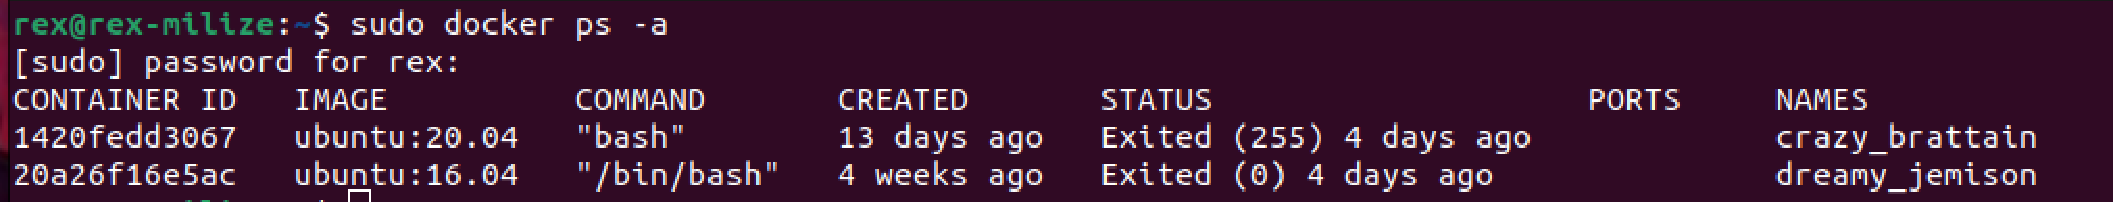
\includegraphics[width=0.85\textwidth]{fig/especifico_2/retornos_de_comandos/sudo_docker_ps_a.pdf}
    \caption{Retorno del comando \ref{lst:docker_basics_ps-a}}
    \label{fig:sudo_docker_ps_a}
\end{figure}

Una vez generados los dos contenedores, los mismos podrán ser consultados mediante el comando que se muestra en \ref{lst:docker_basics_ps-a}, este se encarga de devolver una lista como la que se muestra en \ref{fig:sudo_docker_ps_a}, donde se puede observar de izquierda a derecha las columnas denominadas: Container ID, el cual es el identificador del contenedor, este valor se debe de utilizar para referirse al contenedor para las operaciones que se realizan fuera del entorno, también se muestra la Imagen que el contenedor tiene instalada, el comando de creación del mismo, la creación del contenedor, el status, los puertos definidos y el Nombre.

Para efectos de este proyecto se tomará importancia solamente a las columnas de (Container ID) e (Image).

\begin{lstlisting}[language=bash, caption={Iniciar un contenedor, Docker}, label=lst:docker_basics_start]
    sudo docker start <ID del contenedor>
\end{lstlisting}

\begin{figure}[h!]
    \centering
    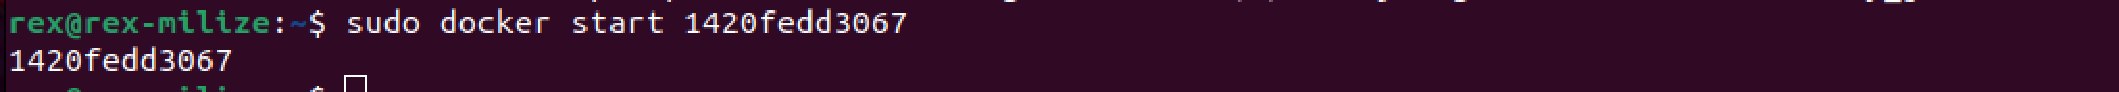
\includegraphics[width=0.85\textwidth]{fig/especifico_2/retornos_de_comandos/sudo_docker_start.pdf}
    \caption{Retorno del comando \ref{lst:docker_basics_start}}
    \label{fig:sudo_docker_start}
\end{figure}

Por medio del comando que se muestra en \ref{lst:docker_basics_start} se inicia el contenedor deseado, esto siempre dependerá del ID que se coloque, tras la ejecución de este comando la salida del mismo se puede observar en la Figura \ref{fig:sudo_docker_start}.

\begin{lstlisting}[language=bash, caption={Ingresar a un contenedor, Docker}, label=lst:docker_basics_init]
    sudo docker exec -it <ID del contenedor> \bin\bash
\end{lstlisting}

\begin{figure}[h!]
    \centering
    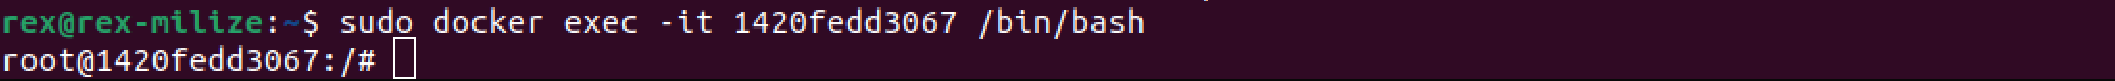
\includegraphics[width=0.85\textwidth]{fig/especifico_2/retornos_de_comandos/sudo_docker_init.pdf}
    \caption{Retorno del comando \ref{lst:docker_basics_init}}
    \label{fig:sudo_docker_init}
\end{figure}

Finalmente, para la ejecución del contenedor en terminal se debe de hacer uso del comando \ref{lst:docker_basics_init}, este se encarga de acceder a la terminal del contenedor deseado. Como se puede observar en la Figura \ref{fig:sudo_docker_init} ya la terminal se encuentra ejecutando el contenedor construido bajo el ID del contenedor "1420fedd3067".

Una vez generados los contenedores, se procede a generar el entorno de desarrollo requerido dentro de los mismos.

\subsubsection{Contenedor para compilación Cruzada}\label{subsec:generacion_entorno_xcompile}

\begin{figure}[h!]
    \centering
    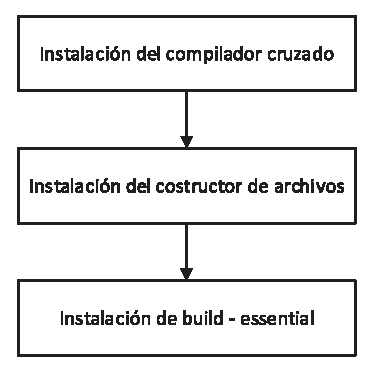
\includegraphics[width=0.85\textwidth]{fig/especifico_2/diagrama_compilador_cruzado.pdf}
    \caption{Diagrama para la elaboración del entorno para compilación cruzada}
    \label{fig:cross_compile_diagram}
\end{figure}

Para la compilación de los archivos se elabora un entorno para compilación cruzada, esto se debe a que el archivo se debera de compilar para la ejecucion en la plataforma de desarrollo seleccionada, es por esto que para la preparacion del entorno se siguen los pasos que se muestran en la Figura \ref{fig:cross_compile_diagram}


\begin{lstlisting}[language=bash, caption={Instalacion del compilador cruzado, Contenedor}, label=lst:cross_compiler]
    sudo apt install gcc-arm-linux-gnueabihf
\end{lstlisting}

\begin{lstlisting}[language=bash, caption={Instalacion de CMake, Contenedor}, label=lst:cmake]
    sudo apt install cmake
\end{lstlisting}

\begin{lstlisting}[language=bash, caption={Instalacion de build essential, Contenedor }, label=lst:build_essential]
    sudo apt install build-essential
\end{lstlisting}

Primeramente se debe de instalar el compilador cruzado, para nuestros efectos será arm-linux-gnueabihf-gcc, esto lo podemos hacer mediante el comando que se muestra en \ref{lst:cross_compiler}. Seguido de esto debemos de instalar CMake el cual es una herramienta de construcción multiplataforma y de código abierto que se utiliza para gestionar la construcción de software, el mismo se instala mediante el comando que se muestra en \ref{lst:cmake}. Finalmente debemos  de instalar build-essential las cuales son herramientas que nos ayudaran a compilar el programa generado, esta instalación se logra mediante el uso del comando mostrado en \ref{lst:build_essential}. Con estas tres instalaciones queda preparado el entorno para la compilación cruzada. 


\subsubsection{Contenedor para Yocto Project}\label{subsec:generacion_entorno_yocto}

\begin{figure}[h!] 
    \centering
    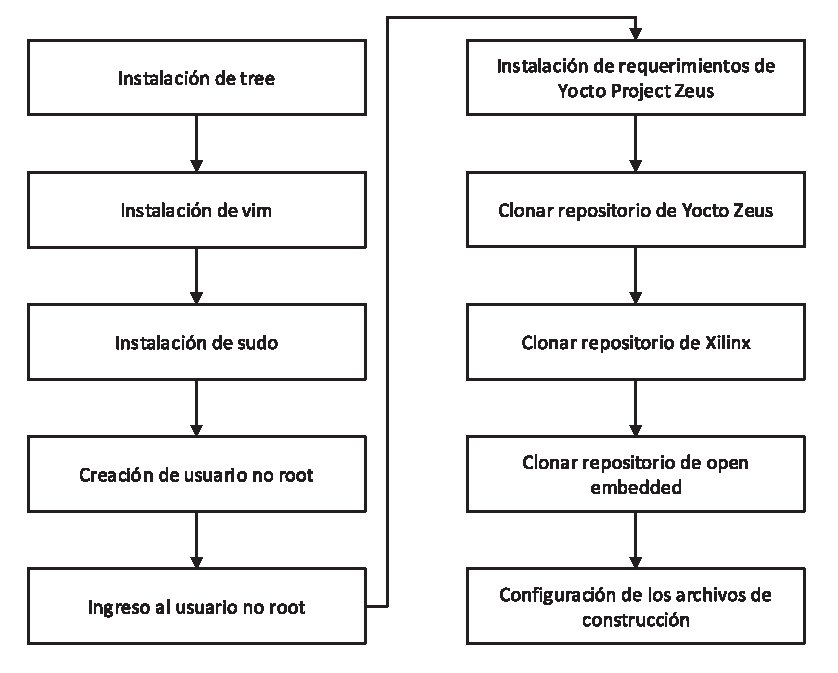
\includegraphics[width=0.85\textwidth]{fig/especifico_2/diagrama_de_entorno_yocto_project.pdf}
    \caption{Diagrama para la elaboración del entorno para Yocto Project}
    \label{fig:yocto_enviroment_diagram_figure}
\end{figure}

El contenedor para Yocto Project, será en el cual se lleve a cabo la construcción de la imagen a utilizar en la plataforma de desarrollo, para esto se requiere la instalación de algunas dependencias las cuales se pueden observar en la Figura \ref{fig:yocto_enviroment_diagram_figure}.



\subsubsection{Creación de un usuario no root}

Para el uso del marco de trabajo de Yocto se debe de generar un usuario no root, esto principalmente por razones de seguridad y manejo adecuado de permisos. El usuario se puede generar por medio de los siguientes comandos:

\begin{lstlisting}[language=bash, caption={Generacion de usuario no root, Linux}, label=lst:no_root_user]
    apt - get install -y sudo
    useradd - ms/bin/bash myuser
    echo "myuser:password" | chpasswd
    usermod - aG sudo myuser
\end{lstlisting}

De forma que según el comando observado en \ref{lst:no_root_user}, en la primera línea instalamos sudo, esto con el fin de poder ejecutar comandos con privilegios de administrador sin tener que iniciar sesión como usuario root, seguido de esto en la segunda línea se agrega el usuario denominado (myuser), en la tercera línea se genera una contraseña para este usuario la cual se define como (chpasswd), finalmente se agrega en el archivo usermod el nuevo usuario el cual, mediante el comando sudo tiene acceso a los privilegios de administrador. 

\begin{lstlisting}[language=bash, caption={Iniciar usuario no root, Linux}, label=lst:no_root_user_log]
    su - myuser
\end{lstlisting}

Cada vez que iniciemos el contenedor siempre lo haremos como usuario root, para poder iniciar con el usuario no root generado en \ref{lst:no_root_user}, se debe de hacer uso del comando que se muestra en \ref{lst:no_root_user_log}, el cual se encarga de iniciar el entorno bajo el usuario llamado (myuser). Cada vez que se realice alguna instalación o procedimiento que requiera permisos de administrador se deberá de ingresar la contraseña.

\subsubsection{Yocto Project}

Como se observó en \ref{subsec:yocto}, yocto presenta flexibilidades a la hora de configurar un sistema permitiendo al desarrollador seleccionar paquetes específicos y personalizar el sistema operativo.

\begin{lstlisting}[language=bash, caption={Requerimientos Yocto Zeus, Linux}, label=lst:yocto_requirements]
    sudo apt - get install gawk wget git - core diffstat unzip texinfo
    gcc - multilib build - essential chrpath socat cpio python python3
    python3 - pip python3 - pexpect xz - utils debianutils 
    iputils - ping python3 - git python3 - jinja2 
    libegl1 - mesa libsdl1 .2 - dev pylint3 xterm
\end{lstlisting}

Para que el mismo funcione de forma correcta debemos de instalar los requerimientos del marco de trabajo los cuales se pueden observar en \ref{lst:yocto_requirements}.

\begin{lstlisting}[language=bash, caption={Version de Yocto}, label=lst:yocto_clone]
    git clone -b zeus https://git.yoctoproject.org/git/poky
    cd poky
\end{lstlisting}

\begin{lstlisting}[language=bash, caption={BSP para Zedboard}, label=lst:yocto_zedboard]
    git clone -b zeus https://github.com/Xilinx/meta-xilinx
    git clone -b zeus https://github.com/openembedded/meta-openembedded.git
\end{lstlisting}

La versión de yocto a utilizar es Yocto Zeus, ya que esta versión es la que contiene soporte para la tarjeta de desarrollo seleccionada, los archivos de esta versión se deben de clonar de \ref{lst:yocto_clone}. Una vez clonado el repositorio se debe de ingresar al directorio (poky) y clonar dentro del mismo el repositorio \ref{lst:yocto_zedboard} el cual contiene la versión de paquete de soporte para la tarjeta requerida, esto con el fin de generar una imagen para la tarjeta de desarrollo seleccionada.

\begin{lstlisting}[language=bash, caption={Configuraciones adicionales, Yocto}, label=lst:aditional_config]
    source oe - init - build - env
    
    echo "MACHINE ??=\"zedboard-zynq7\"" >> conf/local.conf
    echo "IMAGE_FEATURES +=\"package-management\"" >> conf/local.conf
    echo "DISTRO_HOSTNAME =\"zynq\"" >> conf/local.conf
    
    bitbake-layers add-layer ../meta-xilinx/meta-xilinx-bsp/
    bitbake-layers add-layer ../meta-openembedded/meta-oe/
\end{lstlisting}

Una vez clonados los repositorios podemos continuar con algunas configuraciones adicionales que se deben de realizar, con el fin de configurar correctamente el entorno de trabajo, estas se muestran en \ref{lst:aditional_config}. La primera línea se encarga de configurar el entorno de trabajo dentro del directorio llamado (build). Dentro del entorno de trabajo generado en (build) en el directorio llamado (conf) encontramos archivos como lo son el local.conf el cual es un archivo de configuración utilizado por el sistema de compilación BitBake. Este archivo esta escrito en lenguaje de configuración de BitBake, define aspectos importantes como la arquitectura del objetivo, la distribución del sistema las imágenes a crear y las herramientas utilizadas, además de incluir rutas adicionales a capas de Yocto o bien a configuraciones específicas de las recetas. 

Además de esto también nos encontramos con el archivo llamado bblayers.conf, este al igual que local.conf, es un archivo de configuración de BitBake que define las capas que se utilizan durante el proceso de compilación. En este como se mencionó anteriormente se encuentran las rutas de las diferentes capas que el sistema de compilación de Yocto debe usar. Estas capas contienen las recetas y los archivos de configuración que controlan la compilación de paquetes, imágenes y el sistema operativo en general. Cabe destacar que el orden en el que se listan las capas puede ser importante, ya que capas más específicas pueden sobreescribir las configuraciones o recetas de capas más generales.

Una vez comprendidos estos conceptos la línea 3 de \ref{lst:aditional_config} se encarga de agregar la máquina, que en nuestro caso sería la tarjeta de desarrollo ZedBoard de Avnet, la línea 4 se encarga de habilitar la administración de paquetes, esto quiere decir que se asegura que el sistema que se está construyendo incluirá las herramientas necesarias para gestionar paquetes (como instalar, actualizar o eliminar) después de que el sistema haya sido desplegado. La línea 4 es la encargada de establecer el nombre del anfitrión, el sistema operativo generado tendrá el nombre de anfitrión configurado como zynq. Por otro lado, la línea 7 y 8 se encargan de agregar las capas al archivo de bblayers.conf.

Finalizada la configuración básica de los entornos de trabajo se sigue con las siguientes secciones en donde se desarrollaran los casos de estudio con el objetivo de demostrar el funcionamiento del flujo de trabajo propuesto en la Figura \ref{fig:diagrama_flujo_trabajo}.

\section{Caso de estudio 1 - Filtro Básico en MATLAB}

Como caso de estudio se seleccionó una aplicación la cual permite realizar una comparación de resultados antes y después del procesamiento de datos, es por esto que se decidió implementar un filtro básico de tipo paso bajo haciendo uso de los bloques de MATLAB Simulink. 

\begin{figure}[h!]
    \centering
    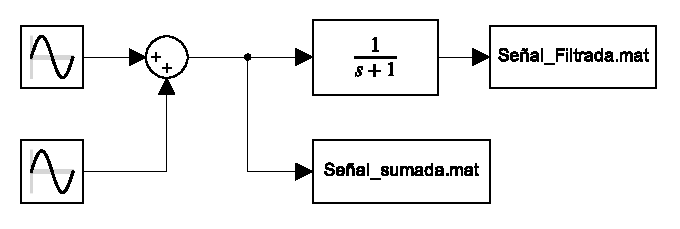
\includegraphics[width=0.5\textwidth]{fig/especifico_2/CASO_ESTUDIO_FILTRO/Diagrama matlab simulink.pdf}
    \caption{Diagrama caso de estudio 1 - Filtro Básico}
    \label{fig:diagrama_matlab_simulink}
\end{figure}

Para la construcción del caso de estudio sé propone el diagrama de la Figura \ref{fig:diagrama_matlab_simulink}, donde para su construcción se llevaran a cabo los siguientes pasos.

\begin{figure}[h!]
    \centering
    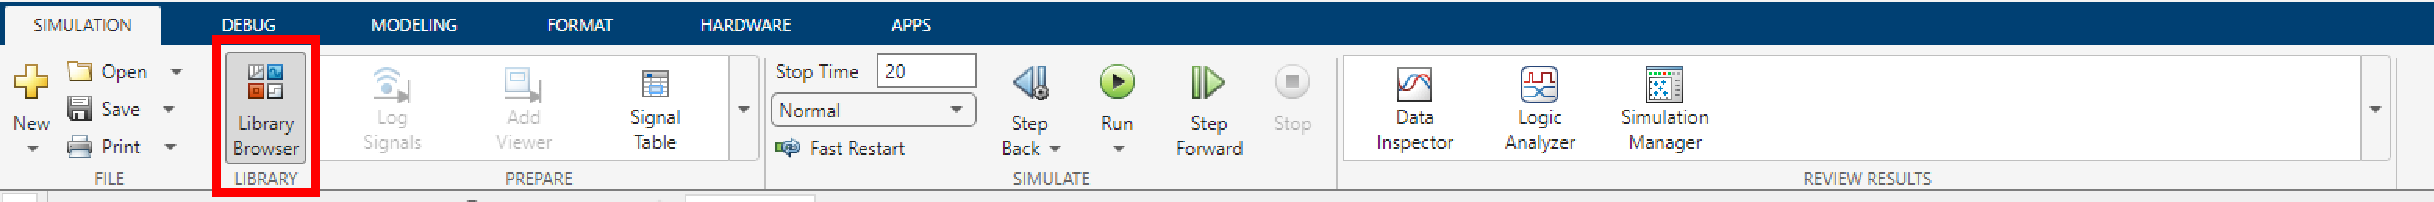
\includegraphics[width=0.8\textwidth]{fig/especifico_2/CASO_ESTUDIO_FILTRO/libbroswer_0.pdf}
    \caption{Librería de bloques}
    \label{fig:lib_bloq}
\end{figure}

Primeramente se deberá de tener acceso a la librería de bloques, la misma se puede encontrar en la ubicación que se muestra en la Figura \ref{fig:lib_bloq}, a esta se debe de acceder haciendo click en el icono que se encuentra resaltado en la Figura anteriormente mencionada.
\newpage


\begin{figure}[h!]
    \centering
    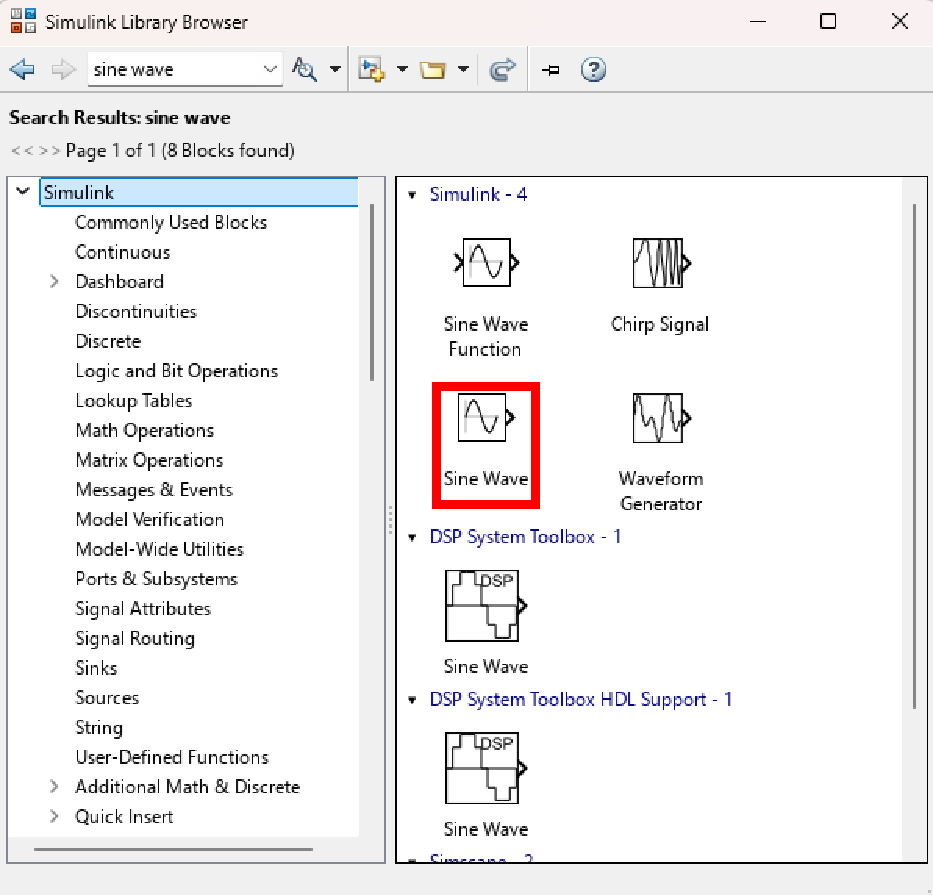
\includegraphics[width=0.5\textwidth]{fig/especifico_2/CASO_ESTUDIO_FILTRO/sinewave_0.pdf}
    \caption{Librería de bloques - generador de onda senoidal}
    \label{fig:lib_bloq_sine}
\end{figure}

Una vez en la librería de bloques, como se puede observar en la Figura \ref{fig:lib_bloq_sine} se debe ingresar en el buscador marcado en color verde la palabra clave del bloque que se desea buscar, para este caso se busca el generador de onda seno del cual se ocupan dos bloques. 

\begin{figure}[htbp]
    \centering
    \begin{subfigure}[b]{0.45\textwidth}
        \centering
        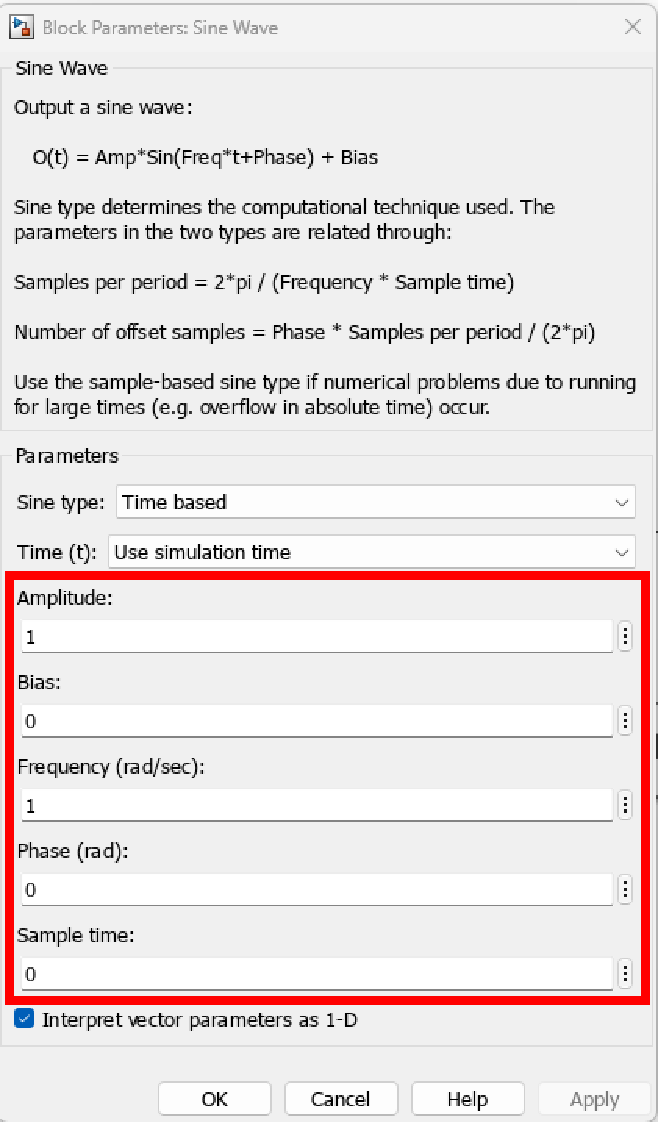
\includegraphics[width=0.7\textwidth]{fig/especifico_2/CASO_ESTUDIO_FILTRO/sinewave_1.pdf}
        \caption{Generador de onda seno 1}
        \label{fig:sine_gen_01}
    \end{subfigure}
    \hfill
    \begin{subfigure}[b]{0.45\textwidth}
        \centering
        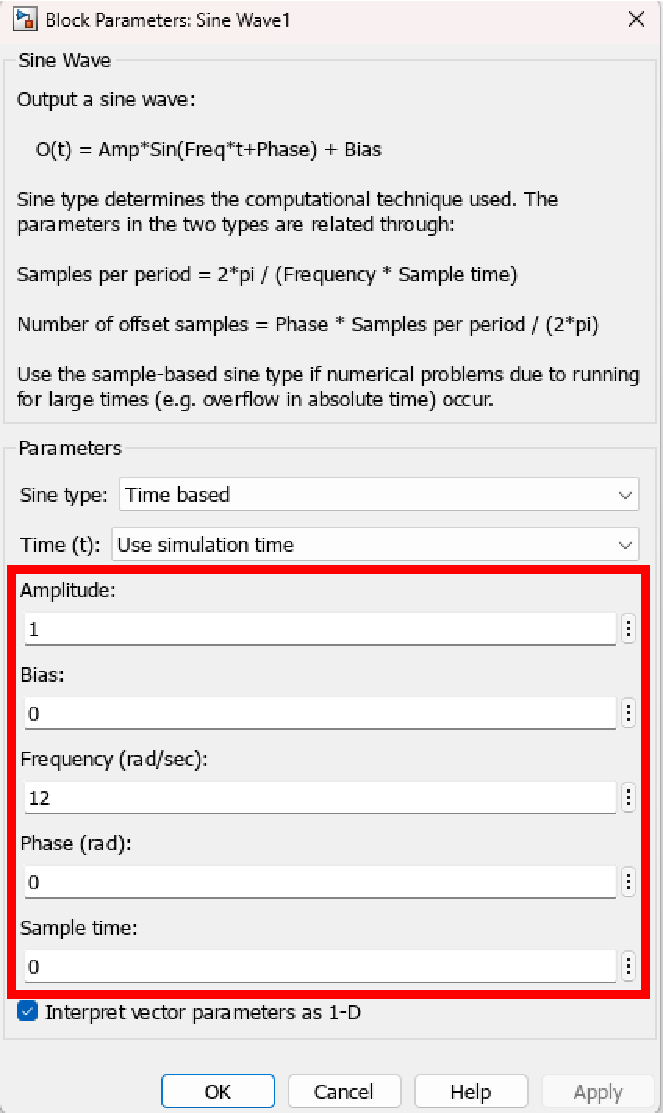
\includegraphics[width=0.7\textwidth]{fig/especifico_2/CASO_ESTUDIO_FILTRO/sinewave_2.pdf}
        \caption{Generador de onda seno 2}
        \label{fig:sine_gen_02}
    \end{subfigure}
    \caption{Configuración de los generadores de onda senoidal}
    \label{fig:sine_wave_generators_config}
\end{figure}

Para la configuración de los generadores de onda senoidales se deben de seguir las configuraciones que se muestran en la Figura \ref{fig:sine_wave_generators_config}, de forma que al primer bloque generador de onda seno se le debe colocar la configuración que se muestra en \ref{fig:sine_gen_01} y al segundo la que se muestra en \ref{fig:sine_gen_02}. De esta forma quedan configurados los bloques encargados de generar las ondas según los parámetros indicados.


\begin{figure}[h!]
    \centering
    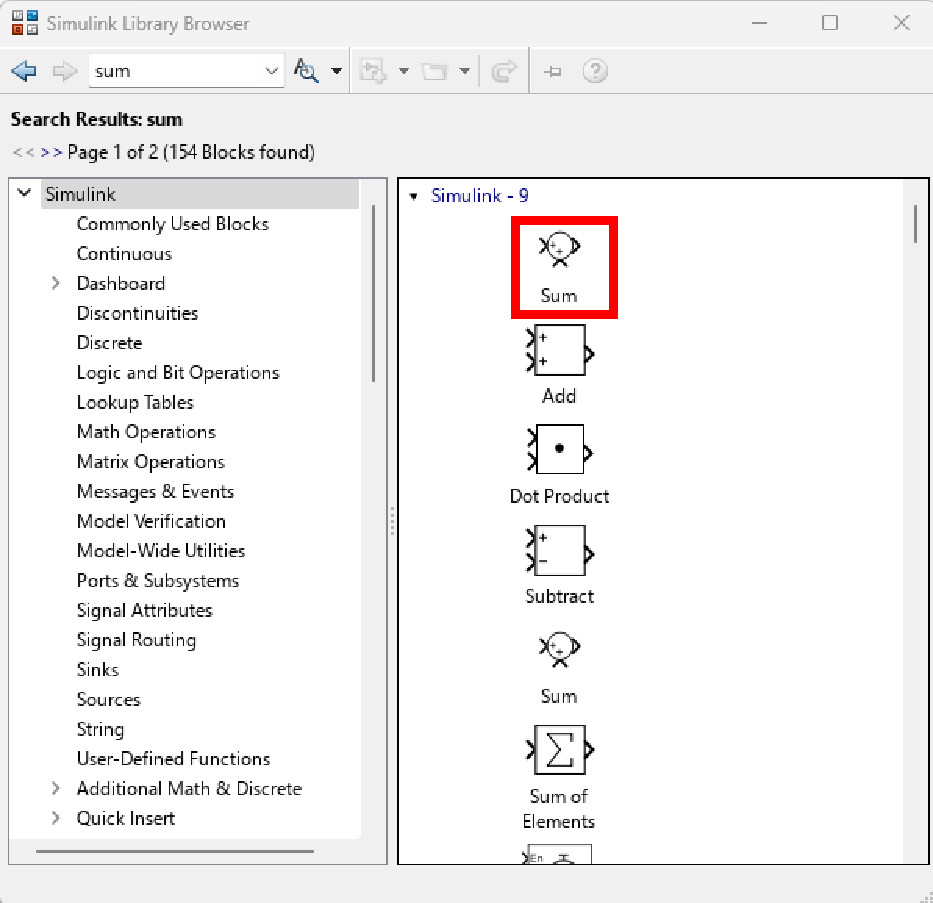
\includegraphics[width=0.5\textwidth]{fig/especifico_2/CASO_ESTUDIO_FILTRO/sum_0.pdf}
    \caption{Librería de bloques - sumador de señales}
    \label{fig:lib_bloq_sum}
\end{figure}

\begin{figure}[h!]
    \centering
    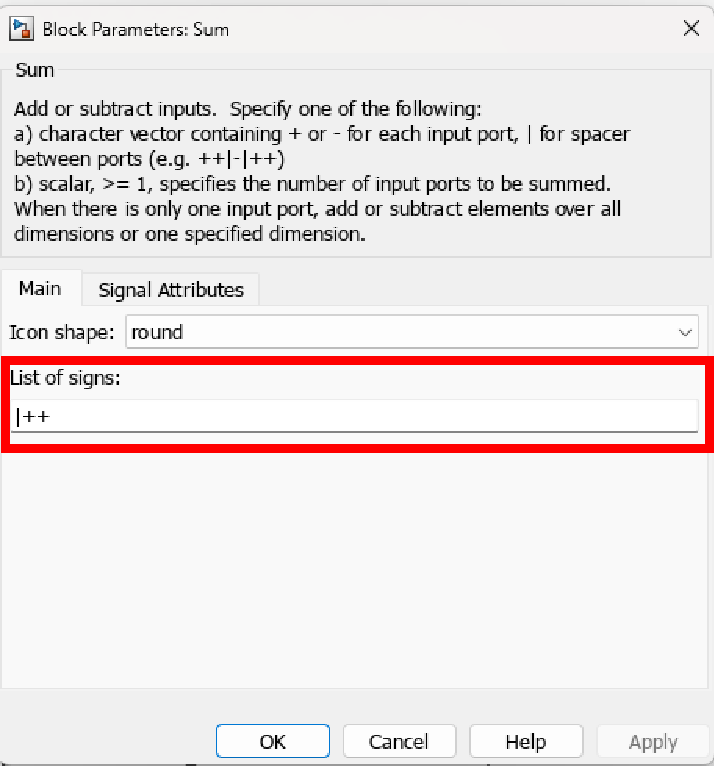
\includegraphics[width=0.5\textwidth]{fig/especifico_2/CASO_ESTUDIO_FILTRO/sum_1.pdf}
    \caption{Configuración del bloque sumador de señales}
    \label{fig:lib_bloq_sum_conf}
\end{figure}


Seguido de esto se debe de implementar el bloque sumador el cual se muestra en la Figura \ref{fig:lib_bloq_sum}, este mismo se debe de configurar como se muestra en la Figura \ref{fig:lib_bloq_sum_conf}, este bloque nos ayudara a sumar las dos señales senoidales, ya que al sumar ondas de diferentes frecuencias, se puede observar un fenómeno llamado modulación, donde la onda resultante presenta un patrón que varía en el tiempo.

\begin{equation}
    y(t) = \sin(t) + \sin(12t)
    \label{eq:funcion_de_suma_de_ondas}
\end{equation}
\newpage

Por otro lado la función de transferencia a utilizar en el filtro será:

\begin{equation}
    H(S) = \frac{1}{S+1}
    \label{eq:funcion_de_transferencia_filtro}
\end{equation}

\begin{figure}[htbp]
    \centering
    \begin{subfigure}[b]{0.45\textwidth}
        \centering
        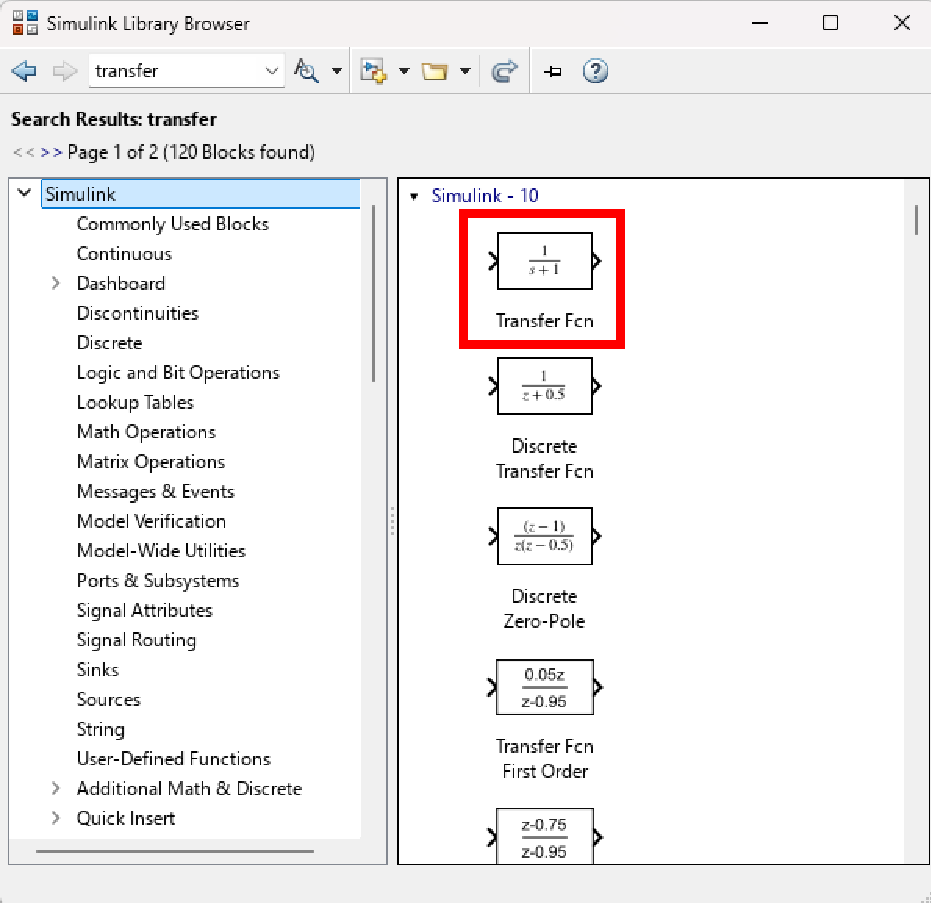
\includegraphics[width=0.9\textwidth]{fig/especifico_2/CASO_ESTUDIO_FILTRO/Transfer_func.pdf}
        \caption{Librería de bloques - función de \\ transferencia}
        \label{fig:lib_bloq_transfer_func}
    \end{subfigure}
    \hfill
    \begin{subfigure}[b]{0.45\textwidth}
        \centering
        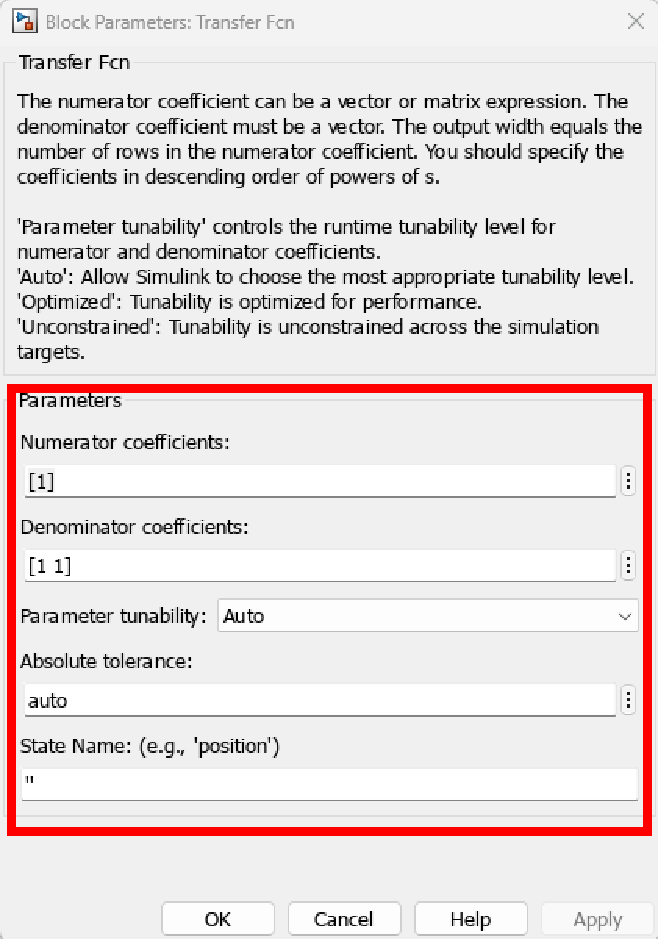
\includegraphics[width=0.7\textwidth]{fig/especifico_2/CASO_ESTUDIO_FILTRO/Transfer_func_1.pdf}
        \caption{Configuración del bloque función de \\ transferencia}
        \label{fig:lib_bloq_transfer_func_conf}
    \end{subfigure}
    \caption{Bloque función de transferencia}
    \label{fig:lib_bloq_transfer_func_all}
\end{figure}

Como se puede observar en la Figura \ref{fig:lib_bloq_transfer_func_all}, podemos observar a la izquierda en \ref{fig:lib_bloq_transfer_func} el bloque de función de transferencia en la librería de bloques, por otro lado a la derecha en \ref{fig:lib_bloq_transfer_func_conf}, podemos observar la configuración que debemos de colocar al mismo, esto con el fin que ejecute la función que se muestra en \ref{eq:funcion_de_transferencia_filtro}. De esta forma al aplicar el filtro a la señal compuesta,  la onda $\sin(t)$ pasará a través del filtro con poca atenuación, mientras que la onda $\sin(12t)$ será significativamente atenuada debido a su  alta frecuencia.

Estos bloques mencionados anteriormente se colocan como se muestra en la Figura \ref{fig:diagrama_matlab_simulink} de modo que se obtienen como salida del sistema dos archivos, uno llamado señal sumada el cual contiene los datos crudos de la modulación de las dos señales senoidales y otro denominado señal filtrada el cual contiene los datos de la señal filtrada por la función de transferencia.

\newpage

\subsection{Simulación del caso de estudio en MATLAB Simulink}\label{subsec:simulacion_caso_de_estudio}

\begin{figure}[h!]
    \centering
    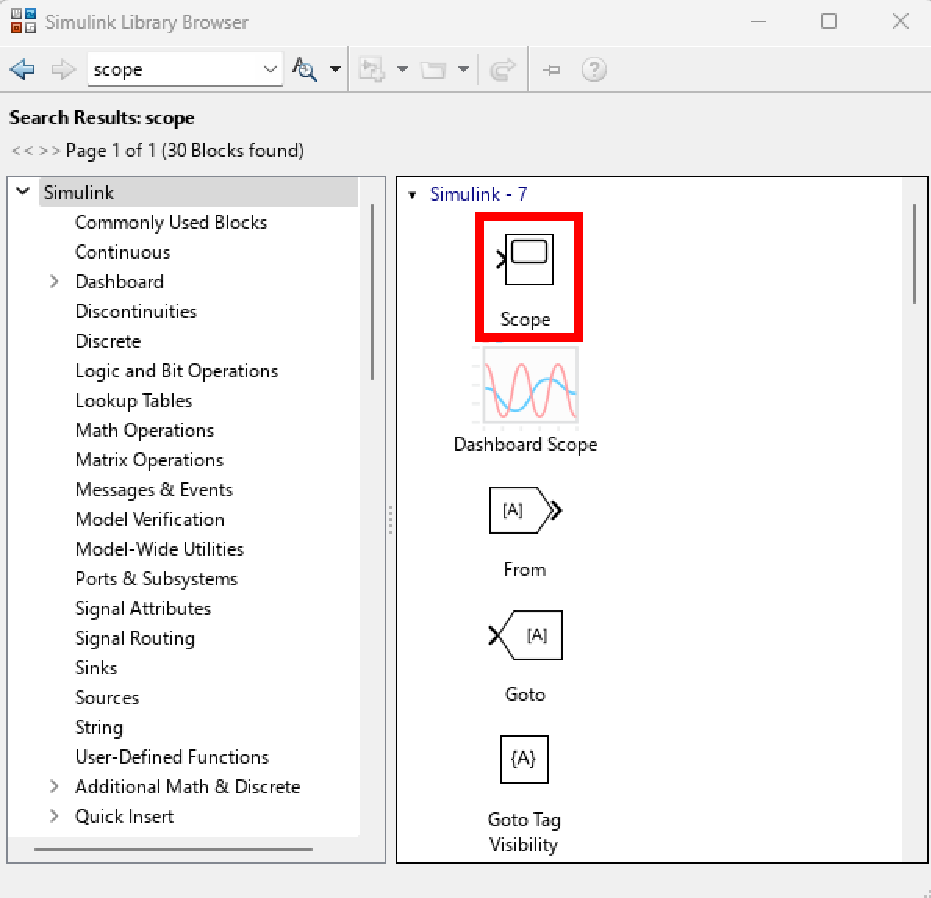
\includegraphics[width=0.5\textwidth]{fig/especifico_2/CASO_ESTUDIO_FILTRO/scope_0.pdf}
    \caption{Librería de bloques - gráfico}
    \label{fig:lib_bloq_graph}
\end{figure}

Para la simulación del caso de estudio que se muestra en la Figura \ref{fig:diagrama_matlab_simulink} se requiere un bloque adicional, el cual se encarga de mostrar de forma grafica los resultados de la ejecución, el bloque se muestra en la Figura \ref{fig:lib_bloq_graph}.

\begin{figure}[h!]
    \centering
    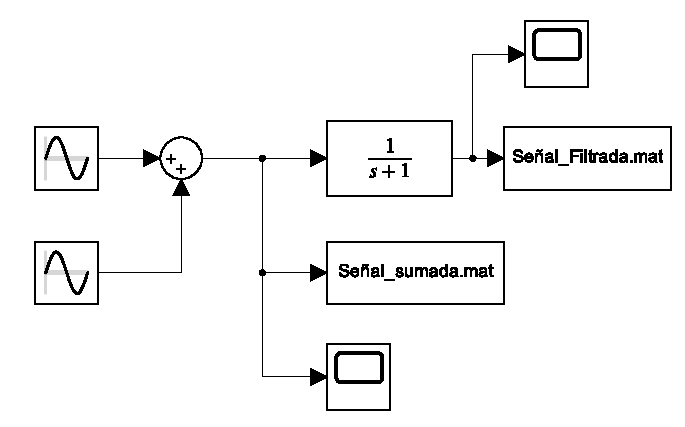
\includegraphics[width=0.5\textwidth]{fig/especifico_2/CASO_ESTUDIO_FILTRO/Diagrama matlab simulink scope.pdf}
    \caption{Diagrama MATLAB Simulink para poder observar las salidas}
    \label{fig:diagrama_matlab_simulink_graficos}
\end{figure}

De esta forma el diagrama de la Figura \ref{fig:diagrama_matlab_simulink}, se colocan dos bloques de gráfico en el diagrama como se muestra en la Figura \ref{fig:diagrama_matlab_simulink_graficos}, esto con el objetivo de poder observar las señales de salida en cada uno de los puntos de interés.


\newpage

\subsubsection{Resultados obtenidos con la ejecución de la simulación}


\begin{figure}[htbp]
    \centering
    \begin{subfigure}[b]{0.45\textwidth}
        \centering
        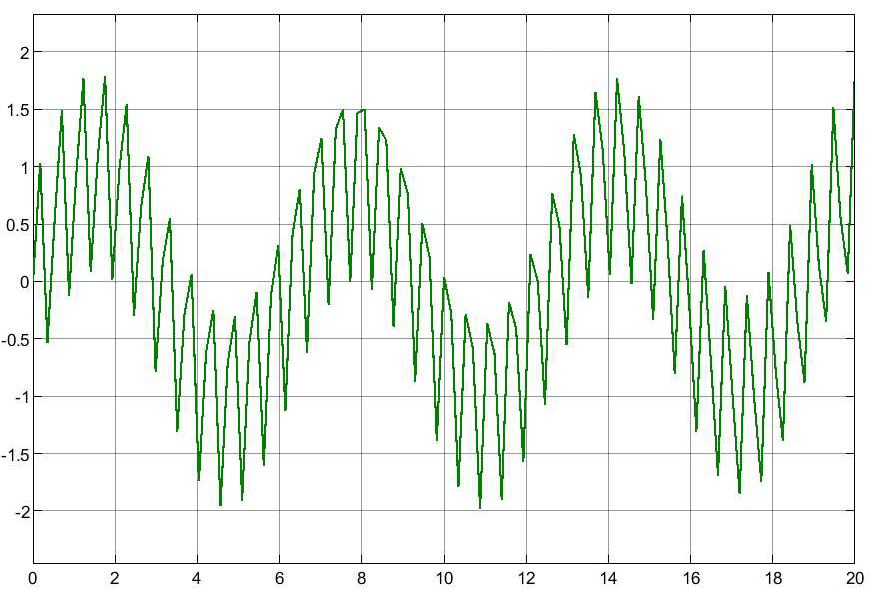
\includegraphics[width=\textwidth]{fig/especifico_2/onda_modulada.pdf}
        \caption{Ondas Moduladas}
        \label{fig:onda_modulada}
    \end{subfigure}
    \hfill
    \begin{subfigure}[b]{0.45\textwidth}
        \centering
        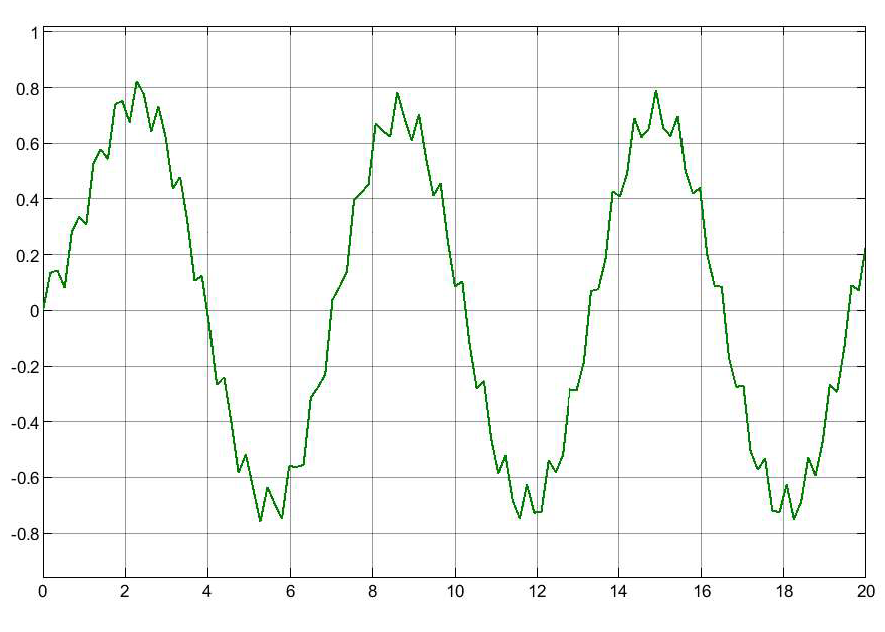
\includegraphics[width=\textwidth]{fig/especifico_2/onda_filtrada.pdf}
        \caption{Onda resultante luego de la función de transferencia}
        \label{fig:onda_filtrada}
    \end{subfigure}
    \caption{Salida simulada del diagrama mostrado en la Figura \ref{fig:diagrama_matlab_simulink_graficos}}
    \label{fig:salida_resultante_diagrama_graficos}
\end{figure}


En la Figura \ref{fig:onda_modulada} se puede observar la modulación de las dos señales senoidales, por otro lado en la Figura \ref{fig:onda_filtrada} se puede observar la salida de la función de transferencia. Siendo la salida esperada de la función de transferencia, ya que al ser un filtro paso bajo atenúa las señales que estén por debajo de la frecuencia de corte, que para este filtro es de 1 $rad/s$. Como la señal compuesta contiene una onda seno con frecuencia de 1 $rad/s$ y otra con frecuencia de 12 $rad/s$ es posible observar aun componentes de la frecuencia atenuada.

\section{Flujo de trabajo de la aplicación de transformación de modelo a modelo}

Para poder cumplir con el objetivo de embeber el sistema, se debe de hacer uso de la herramienta MATLAB Simulink Coder. Como se mencionó en \ref{sec:modelo2model}, a este tipo de aplicaciones se les conoce como transformadores de modelos, en este caso se emplea para lograr transformar el diagrama de control implementado en MATLAB Simulink en un código de lenguaje C, manteniendo de esta forma la estructura del modelo, pero realizando una adaptación al formato requerido, este convertidor de modelos garantiza la consistencia del modelo de control además de realizar la adaptación del mismo a las características de la tarjeta de desarrollo ZedBoard. Algunos de los parámetros que se pueden configurar en este transformador de modelos son: parámetros de la solución, implementación en hardware y generación de código.
\newpage

\begin{figure}[h!]
    \centering
    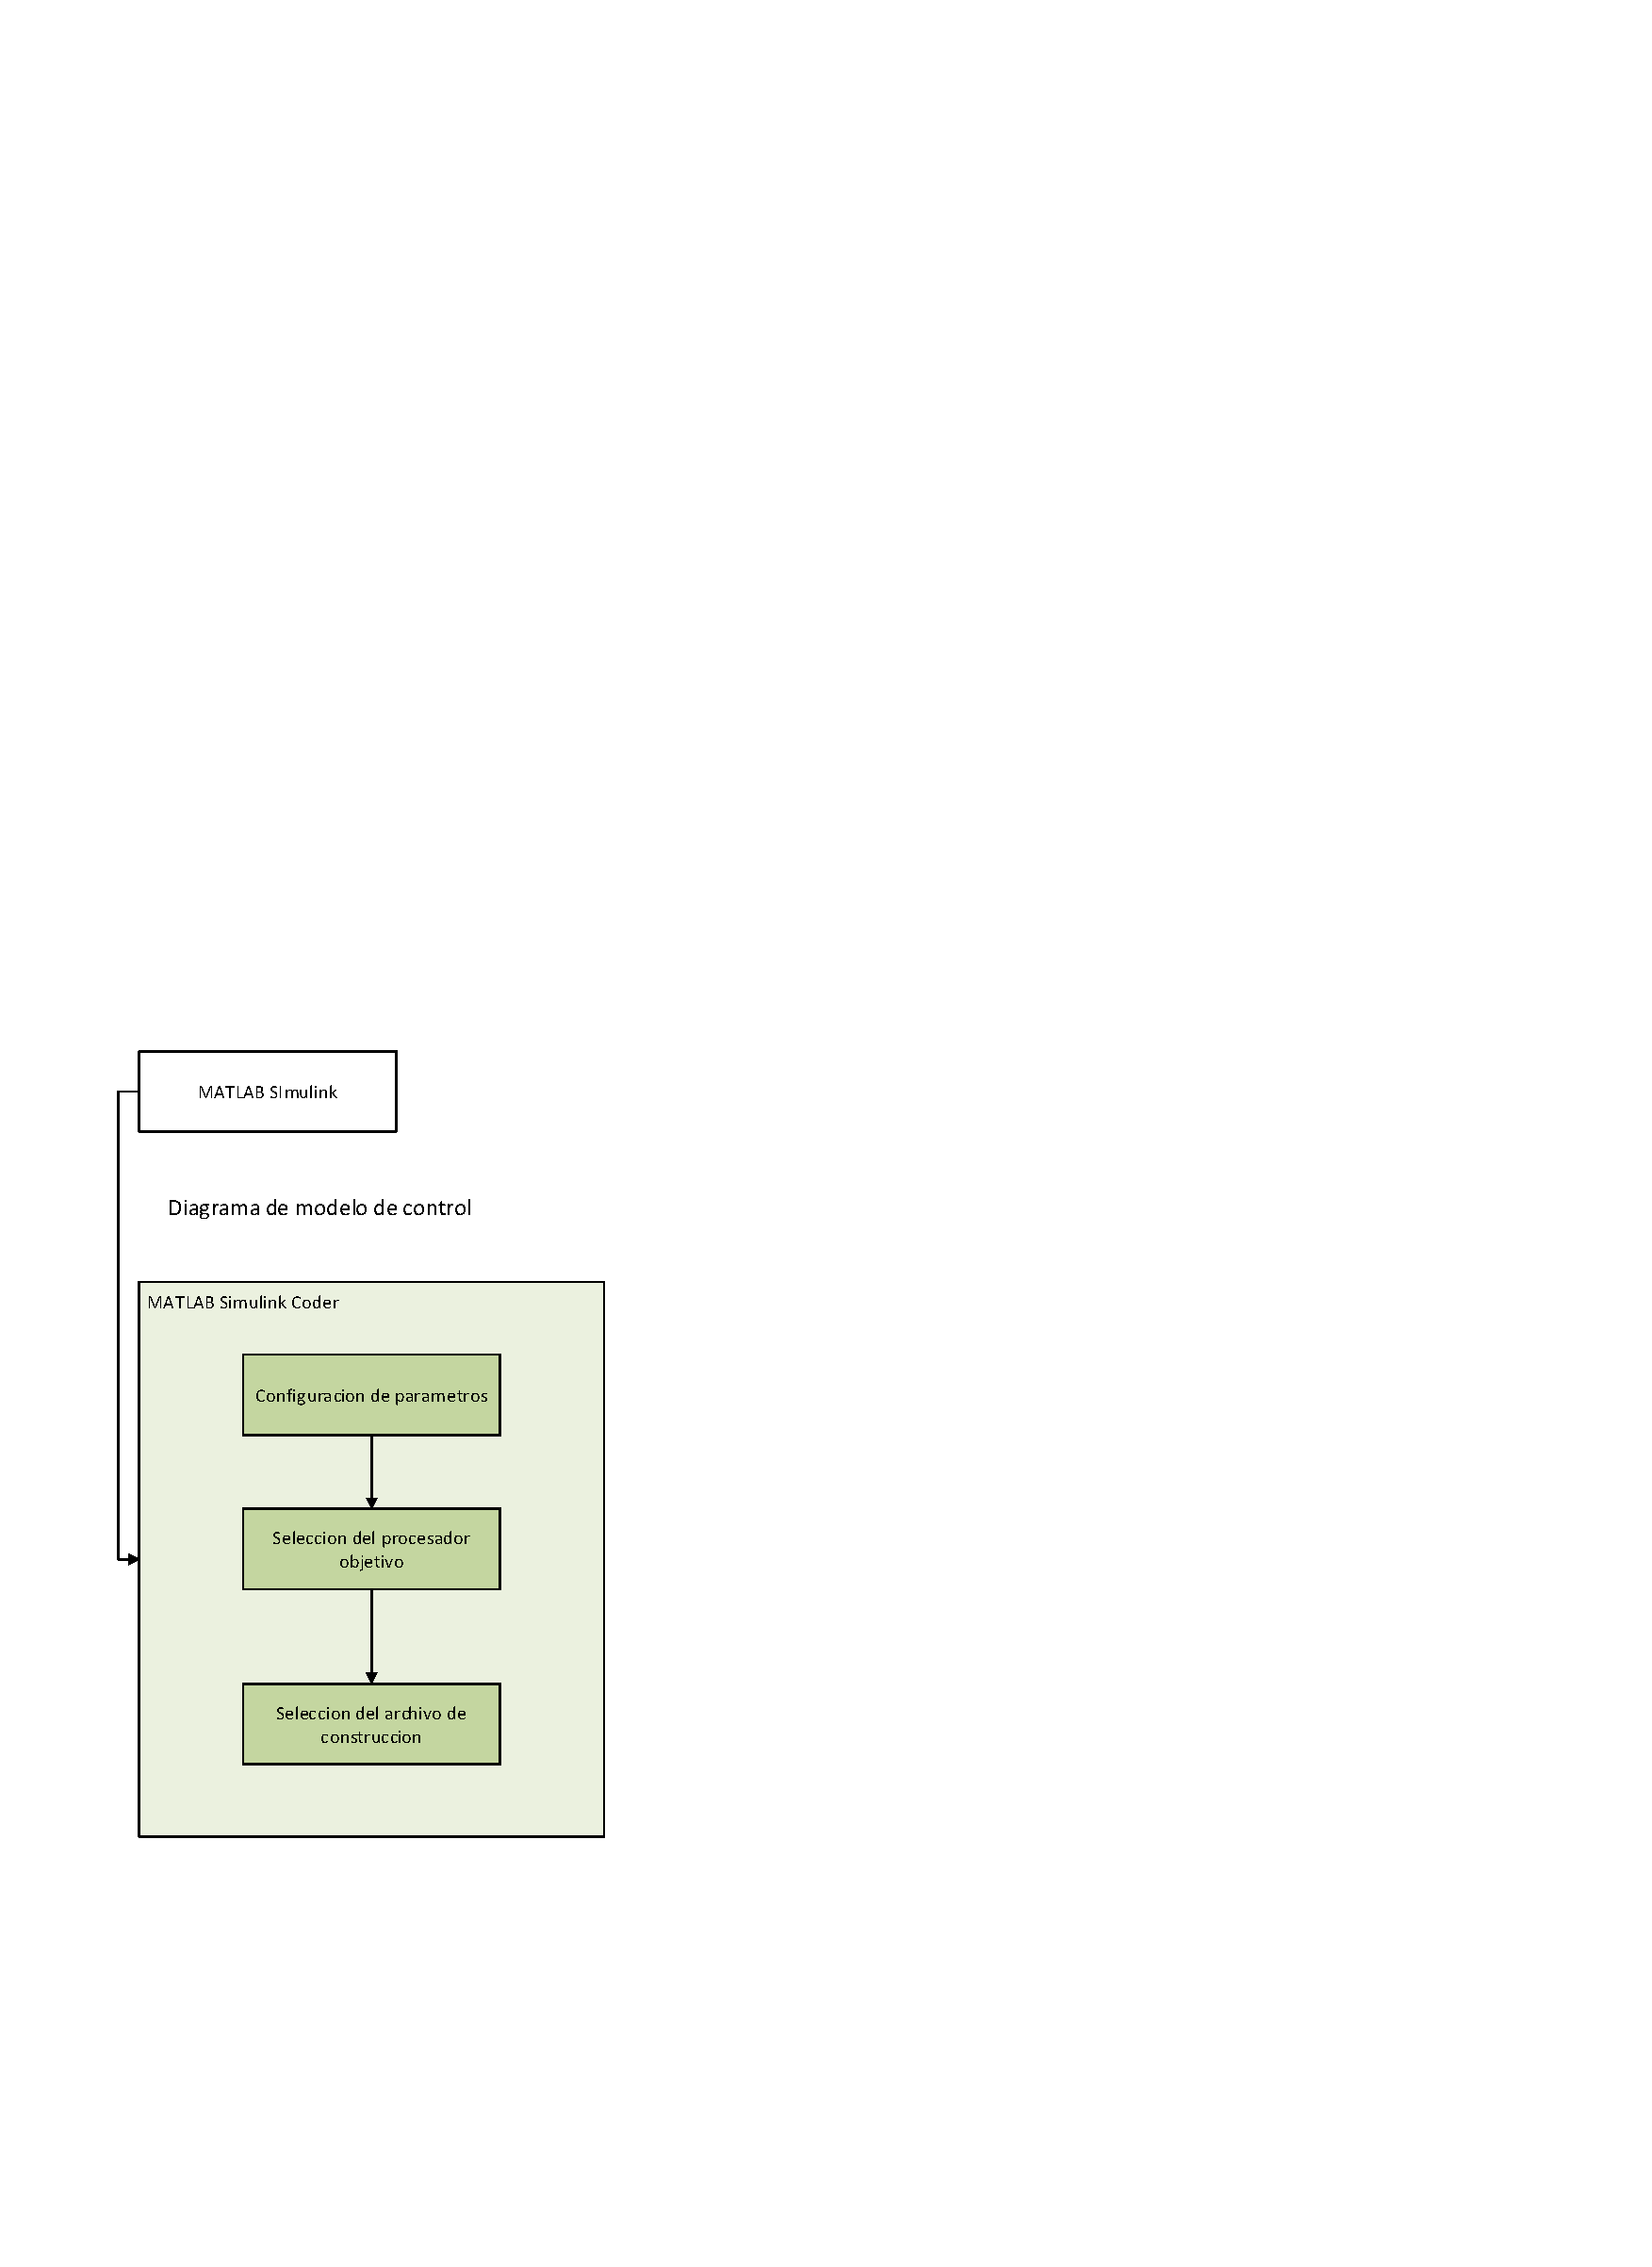
\includegraphics[width=0.8\textwidth]{fig/especifico_2/M2MT/model_2_model_diagram.pdf}
    \caption{Flujo de trabajo MATLAB Simulink Coder}
    \label{fig:m2m_matlab_simulink_coder}
\end{figure}

En la Figura \ref{fig:m2m_matlab_simulink_coder} se puede encontrar un diagrama que contempla los pasos a seguir en esta sección, los cuales se explicaran a lo largo de este capítulo, además, se definirán los parámetros que se deben de utilizar y el funcionamiento de estos dentro de la generación del código C.

\subsection{Simulink Coder}\label{subsec:simulink_coder}

Una vez comprobado el comportamiento esperado por el caso de estudio mediante la simulación, se puede proceder con la ejecución del flujo de trabajo de MATLAB Simulink Coder, esto con el fin de transformar el modelo generado en MATLAB Simulink a un modelo de lenguaje de programación C. Cabe destacar que para esta implementación se utilizó el diagrama que se muestra en la Figura \ref{fig:diagrama_matlab_simulink}, ya que, este solamente contiene como salida los archivos con los datos numéricos del sistema y no contiene las salidas gráficas agregadas en \ref{subsec:simulacion_caso_de_estudio}.


\subsection{Definición de parámetros}

\begin{figure}[h!]
    \centering
    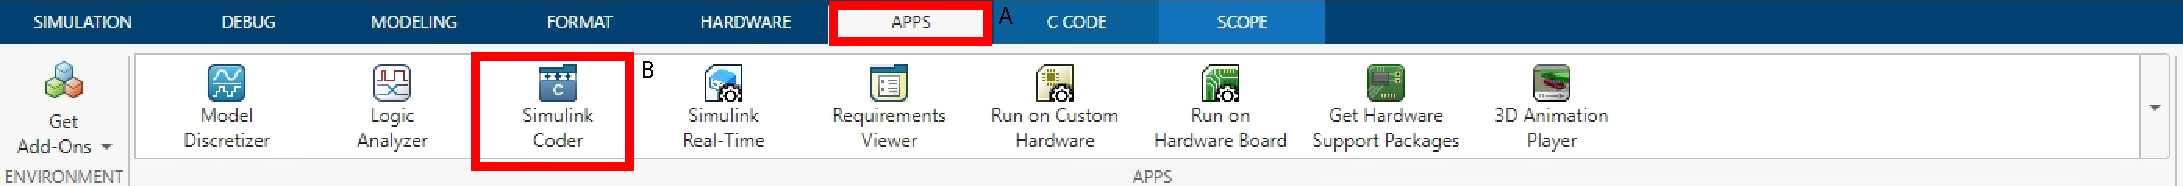
\includegraphics[width=0.8\textwidth]{fig/especifico_2/M2MT/paso_a_paso_mtmt/apps.pdf}
    \caption{Pestaña Aplicaciones}
    \label{fig:pestana_apps}
\end{figure}

\begin{figure}[h!]
    \centering
    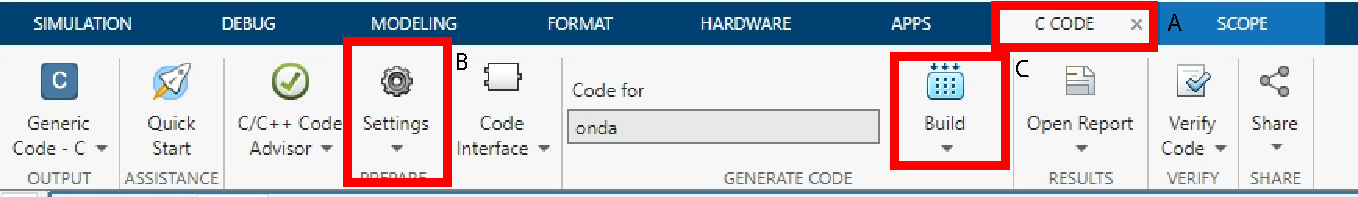
\includegraphics[width=0.8\textwidth]{fig/especifico_2/M2MT/paso_a_paso_mtmt/c_code.pdf}
    \caption{Pestaña código C}
    \label{fig:pestana_c_code}
\end{figure}

\begin{figure}[h!]
    \centering
    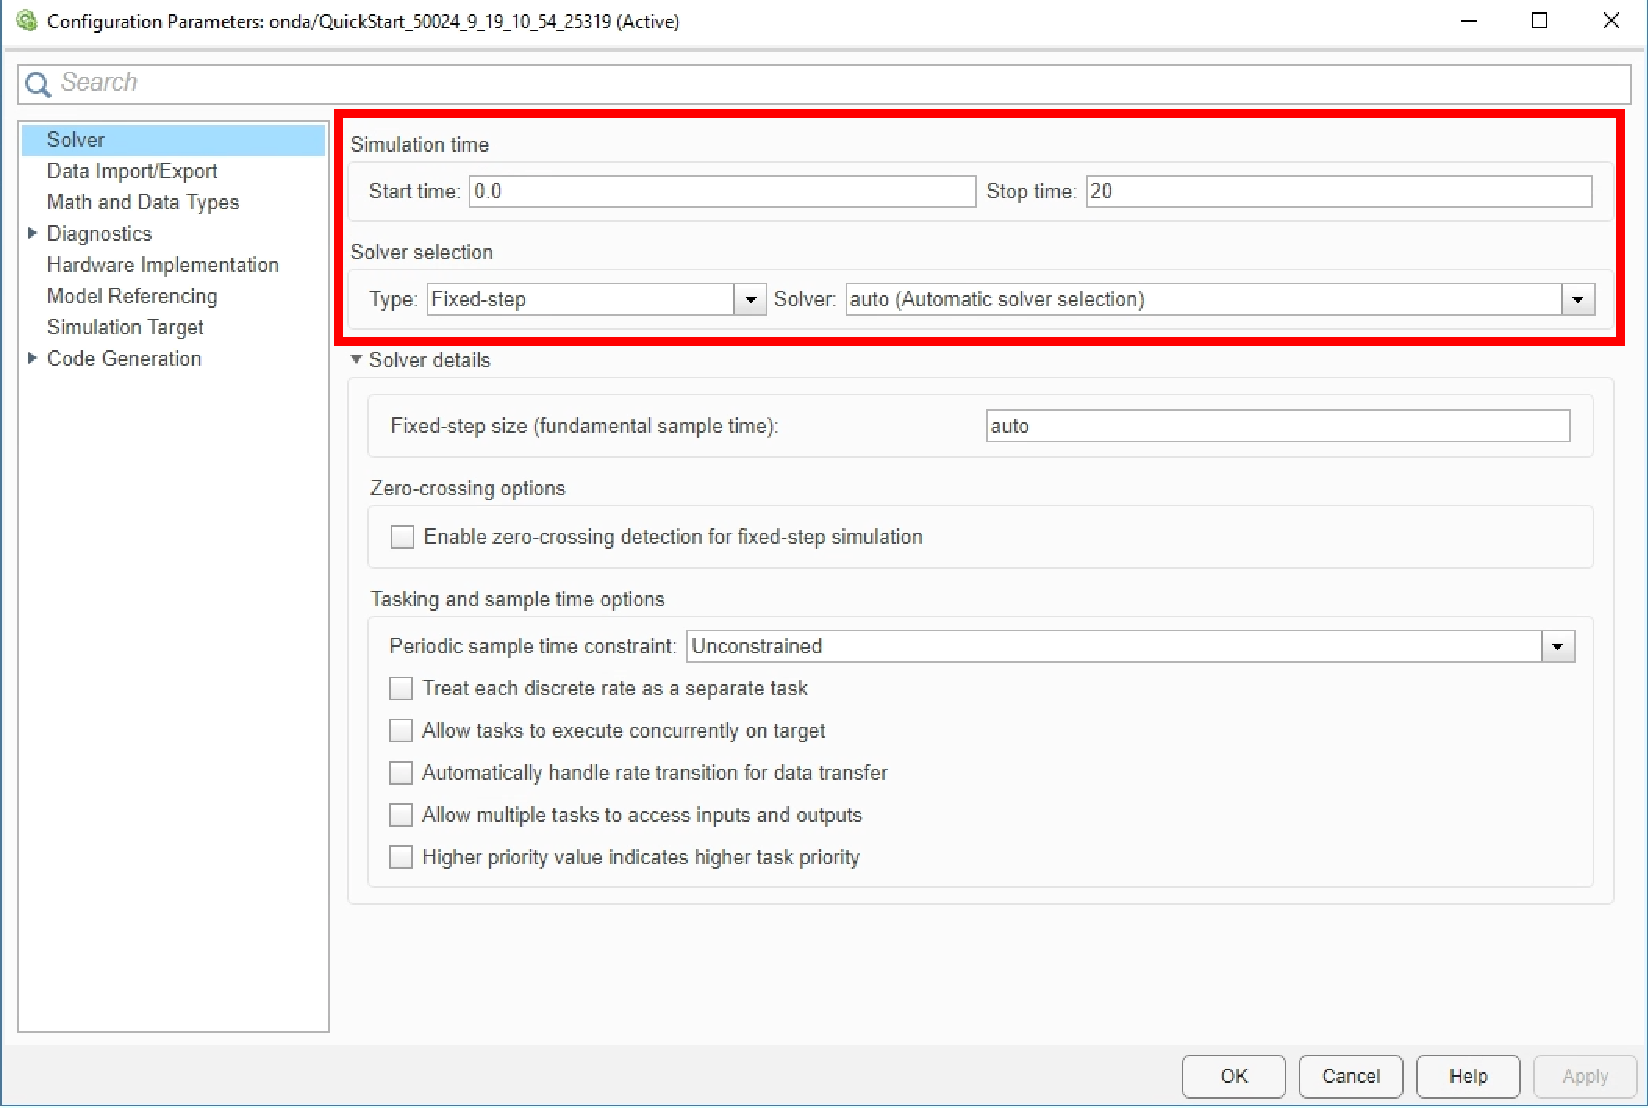
\includegraphics[width=0.8\textwidth]{fig/especifico_2/M2MT/paso_a_paso_mtmt/configuration_parameters.pdf}
    \caption{Configuración de parámetros}
    \label{fig:pestana_config}
\end{figure}

Para la definición de parámetros, se debe de estar en el entorno de MATLAB Simulink, una vez en el entorno mencionado anteriormente se debe ir a la pestaña denominada Aplicaciones, o bien APPS como se muestra en la Figura \ref{fig:pestana_apps}, se deberá de seleccionar la aplicación denominada Simulink Coder, cuando seleccionamos esta opción se abrirá una pestaña llamada código C, o bien C CODE como se pudo observar en la Figura \ref{fig:pestana_c_code}.

Una vez estemos en la pestaña de código C, debemos de ir a la opción de configuración de parámetros, en la Figura \ref{fig:pestana_c_code} se observa esta opción bajo el nombre de settings, una vez presionada la opción se abre una ventana emergente como la que se muestra en la Figura \ref{fig:pestana_config}, en la pestaña denominada Solver se deberán de proporcionar los datos sobre el tiempo de ejecución de la prueba.

\subsubsection{Selección del procesador objetivo}

\begin{figure}[h!]
    \centering
    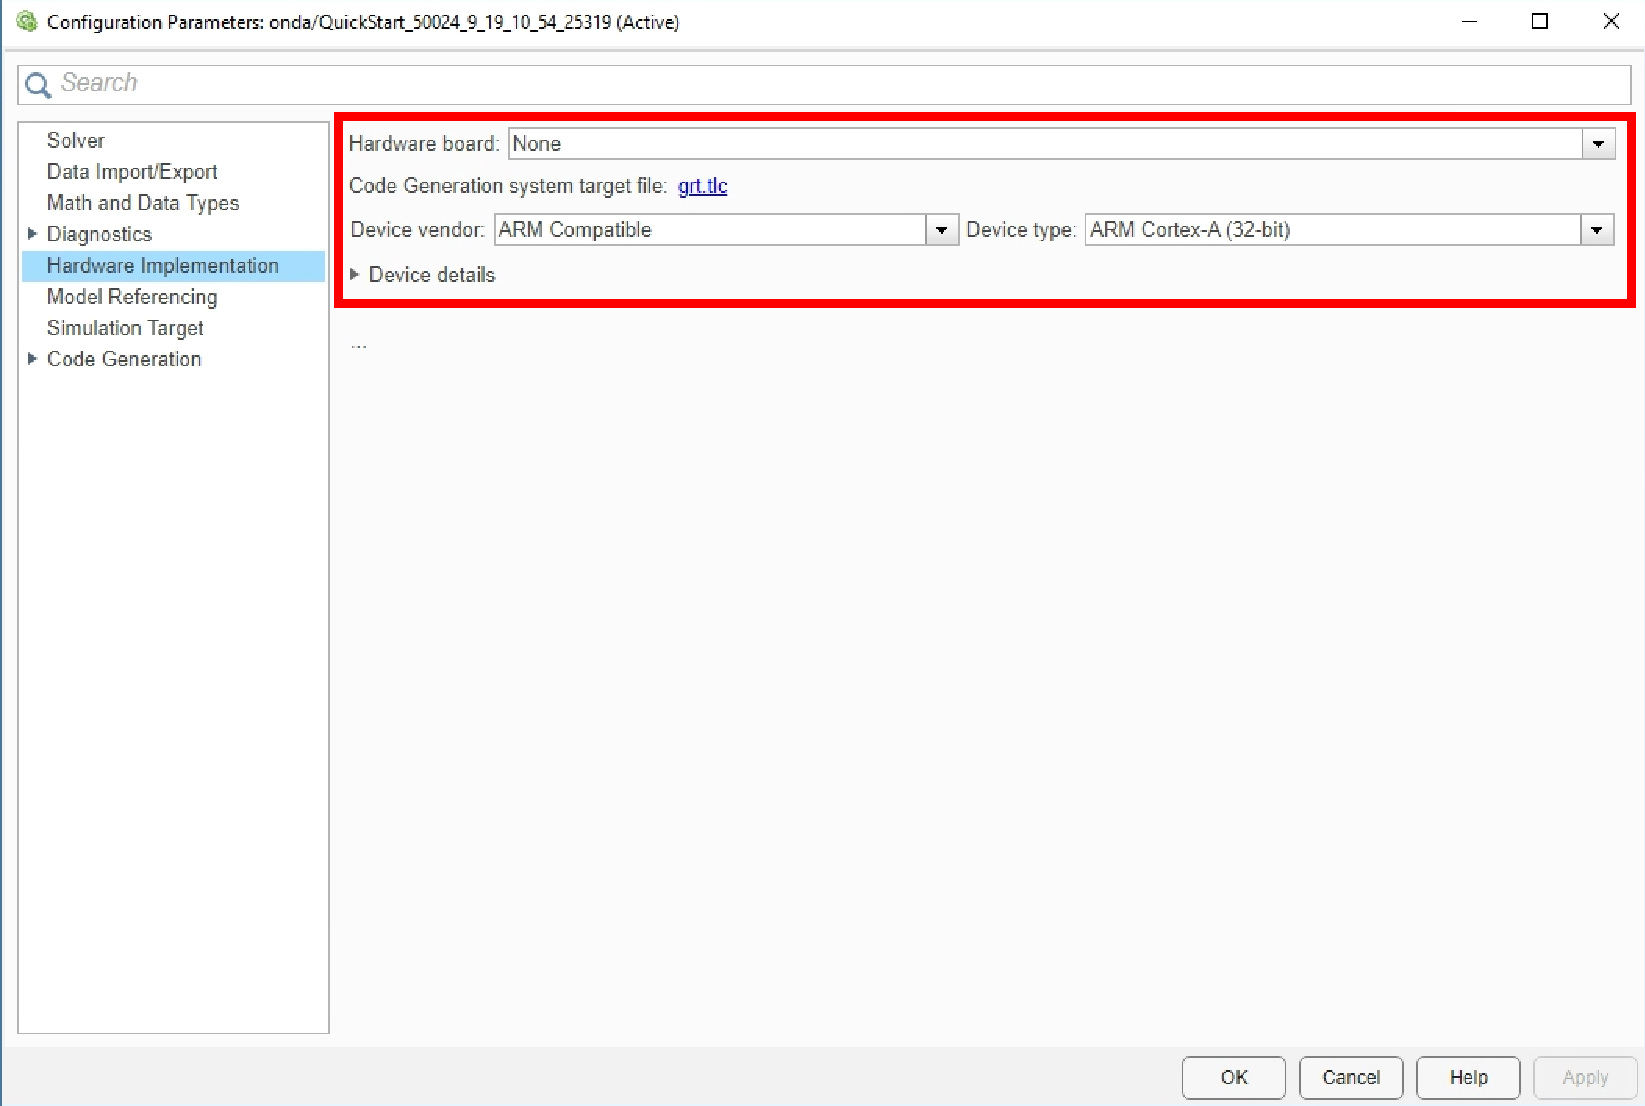
\includegraphics[width=0.8\textwidth]{fig/especifico_2/M2MT/paso_a_paso_mtmt/configuration_parameters_processor.pdf}
    \caption{Selección del procesador y la familia del procesador}
    \label{fig:pestana_config_procesador}
\end{figure}

Continuando en la sección de configuración de parámetros ahora debemos de ir a la pestaña llamada implementación de hardware o bien Hardware Implementation, en donde deberemos de colocar los datos de Device Vendor el cual hace referencia al tipo de procesador que contiene la tarjeta de desarrollo, para nuestro caso sería ARM Compatible y el Device Type que seria a la familia que pertenece el procesador, para nuestro caso sería un ARM Cortex-A de 32-bits tal y como se muestra en la Figura \ref{fig:pestana_config_procesador}.


\subsubsection{Selección del tipo de archivo de construcción}

Anteriormente configuramos los parámetros de tiempo de operación y procesador de la tarjeta de desarrollo, ahora debemos de configurar el tipo de archivo que se utilizara para la generación de los archivos binarios, como se deberá de realizar una compilación cruzada se debe de elegir un tipo de archivo el cual nos permita compilar los binarios para la ejecución del sistema sin importar el sistema operativo de la máquina host. Es por esto que se debe de seleccionar en la pestaña de Code Generation el Toolchain denominado CMake tal y como se muestra en la Figura \ref{fig:pestana_config_output_file}, además de esto se debe de marcar tanto la opción denominada como Generate code only, como Package code and artifacts, esta última nos genera como salida un archivo comprimido con todos los requerimientos de la aplicación para poder ser construida.


\begin{figure}[h!]
    \centering
    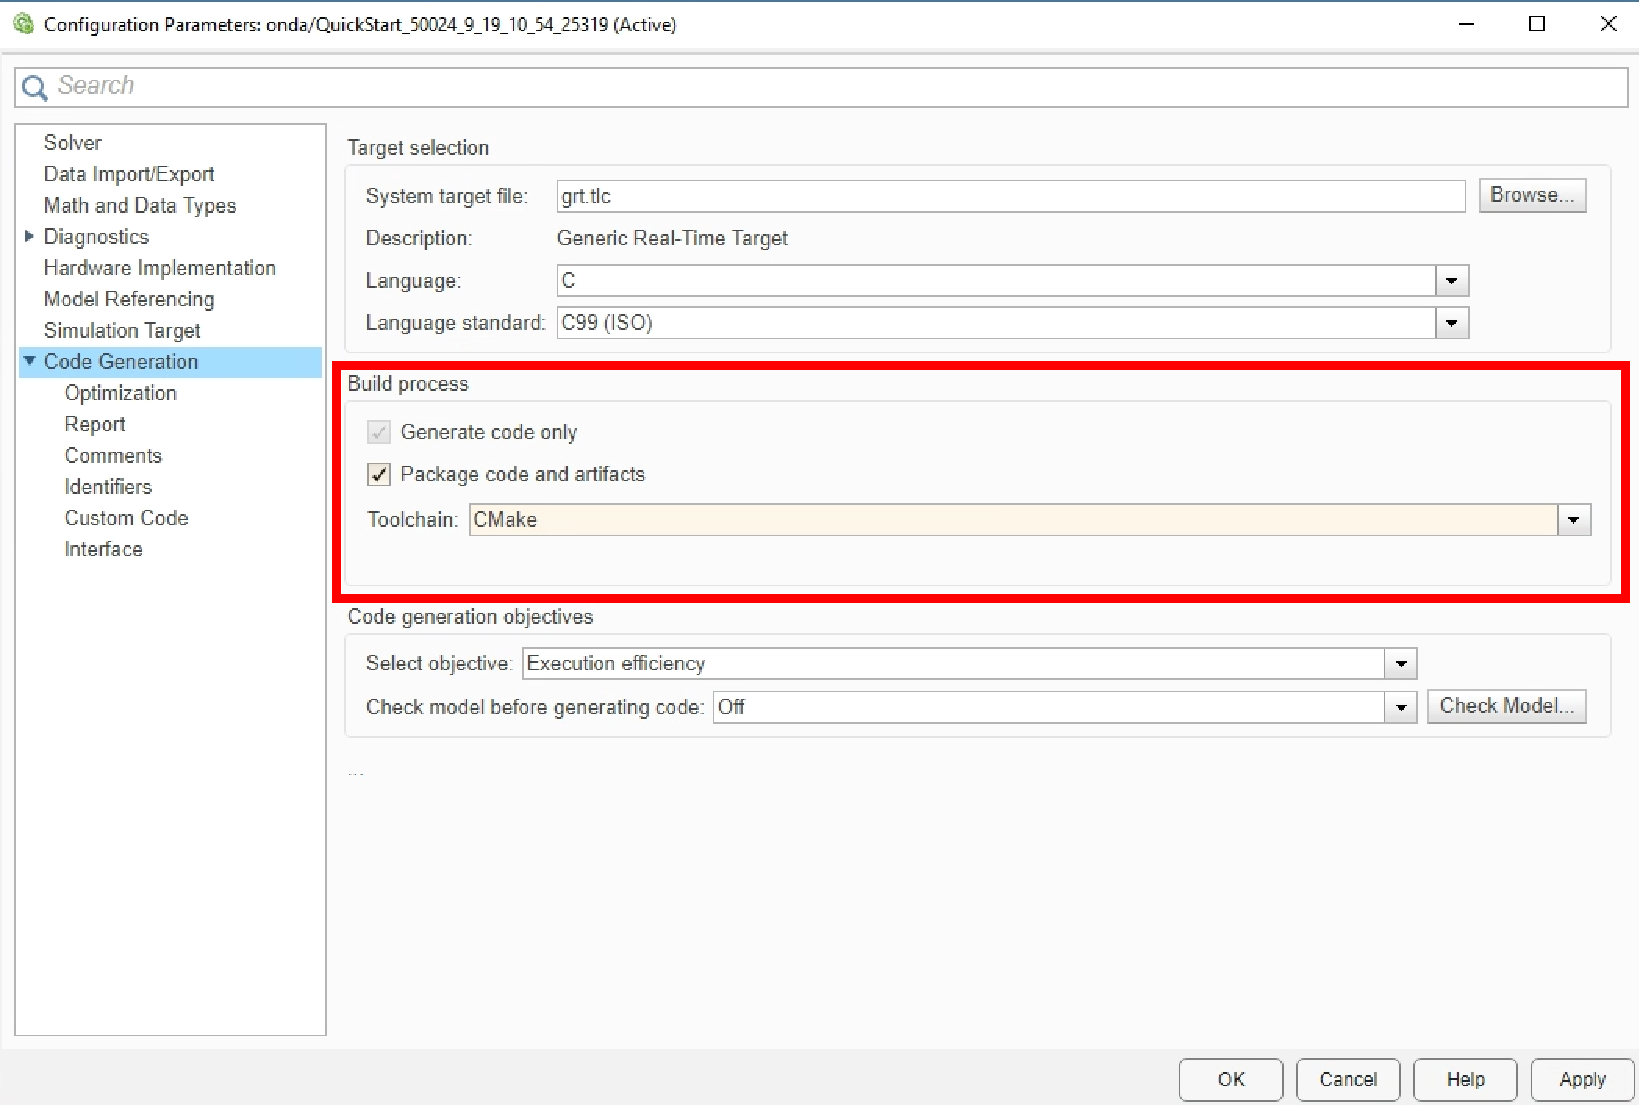
\includegraphics[width=0.8\textwidth]{fig/especifico_2/M2MT/paso_a_paso_mtmt/configuration_output_file.pdf}
    \caption{Selección del tipo de archivo de construcción}
    \label{fig:pestana_config_output_file}
\end{figure}

\subsubsection{Generación de archivos de compilación}

Una vez configurados todos los parámetros mencionados anteriormente debemos de proceder con la construcción de los archivos, para esto se debe de ir a la barra de tareas a la opción denominada como generar código, la misma se puede observar en la Figura \ref{fig:pestana_c_code} bajo el nombre de Build.

\begin{figure}[h!]
    \centering
    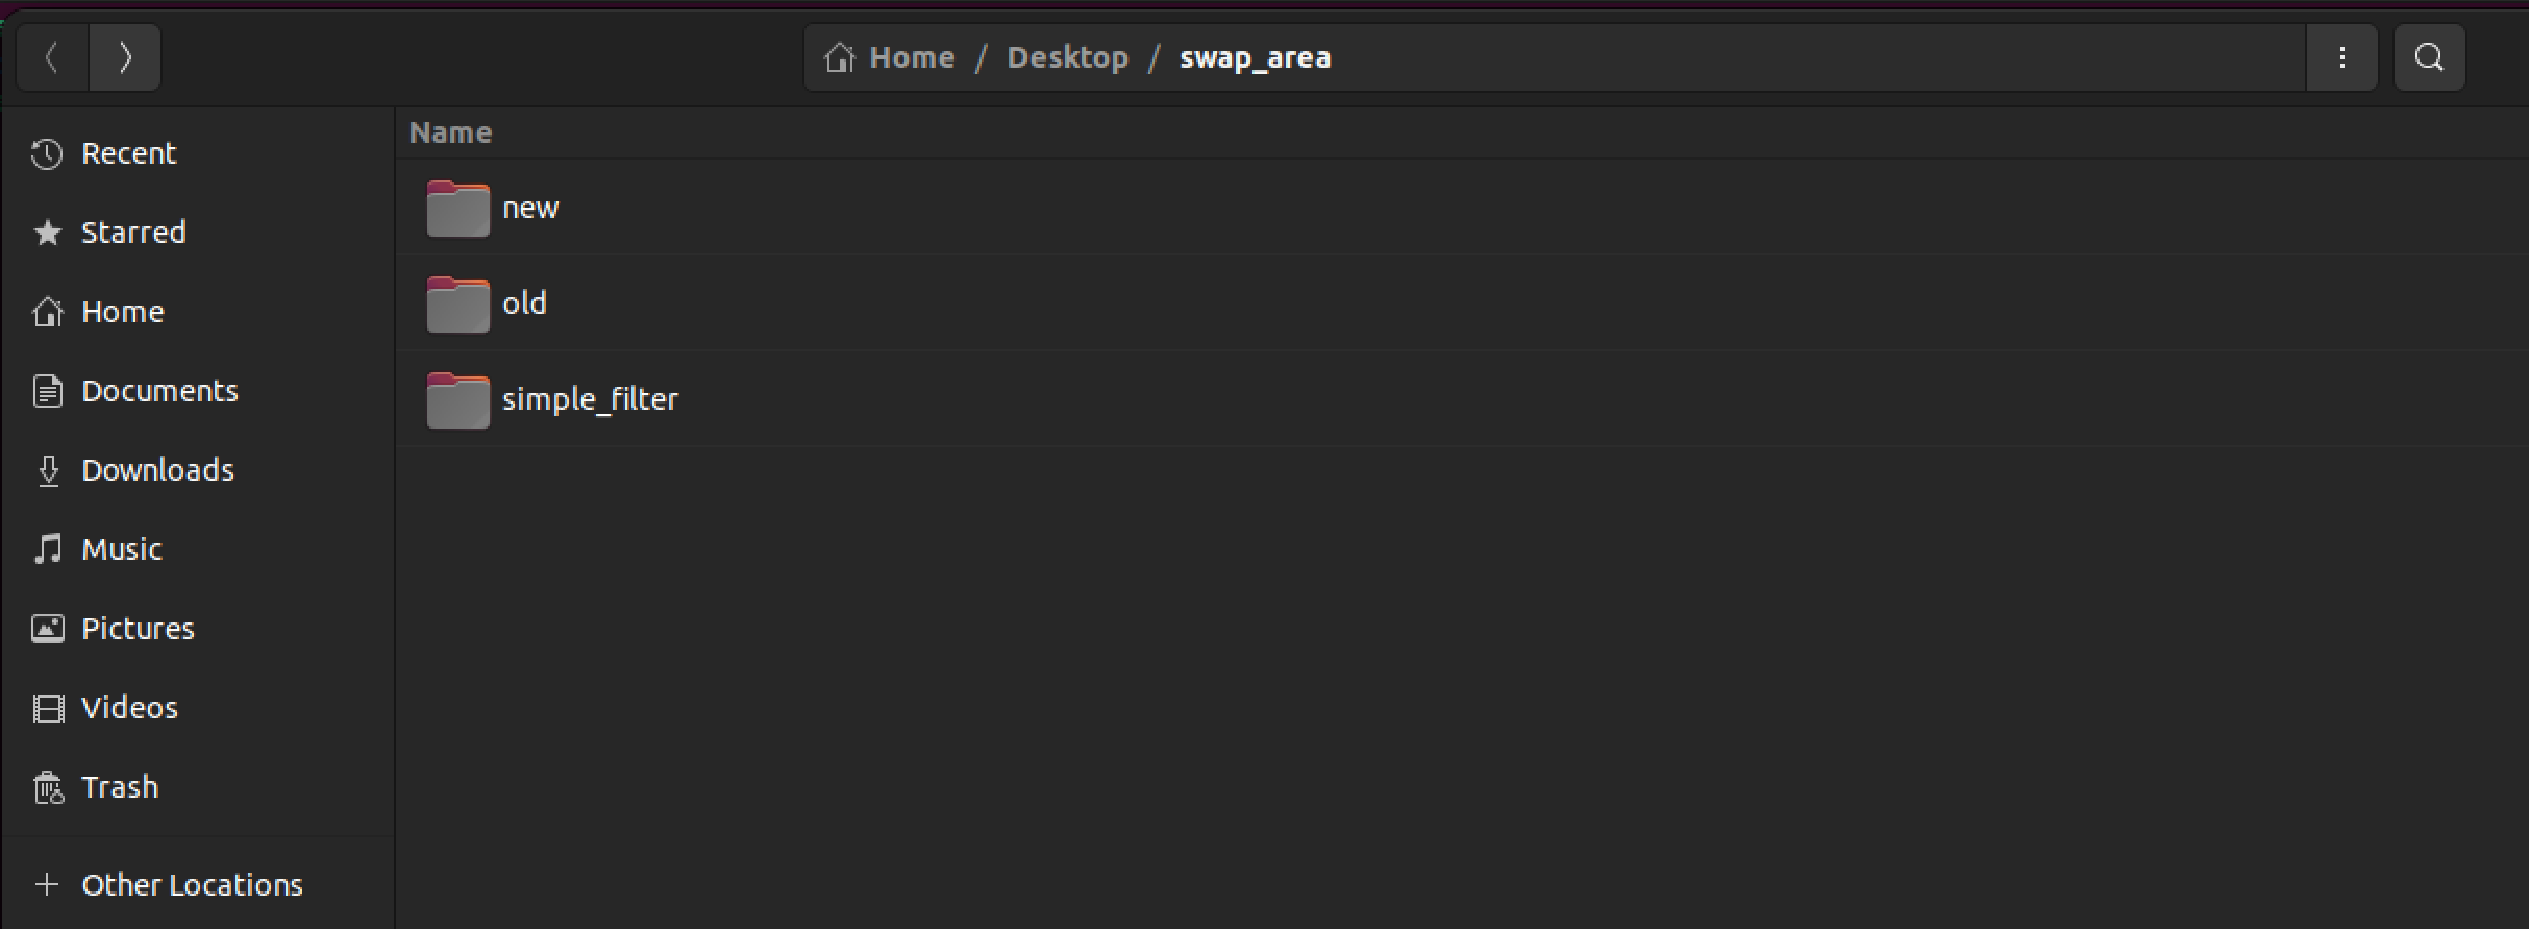
\includegraphics[width=0.8\textwidth]{fig/especifico_2/M2MT/paso_a_paso_mtmt/root_folder.pdf}
    \caption{Archivo comprimido en el directorio swap\_area}
    \label{fig:pestana_swap_area}
\end{figure}

\begin{lstlisting}[language=bash, caption={Copiar archivos al contenedor, Linux}, label=lst:copy_to_container]
    sudo docker cp /direccion/del/archivo 
    <id_de_contenedor>:/direccion/del/contenedor
\end{lstlisting}

\begin{lstlisting}[language=bash, caption={Copiar archivos del contenedor, Linux}, label=lst:copy_from_container]
    sudo docker cp <id_de_contenedor>:/direccion/del/contenedor
    /direccion/del/archivo
\end{lstlisting}

Seguido de esto se debe de copiar el archivo comprimido generado en \ref{subsec:simulink_coder}, al contenedor con Ubuntu 16.04 generado en \ref{sec:entorno_en_contenedores}. Primeramente colocaremos el archivo comprimido en un directorio llamado swap\_area, tal y como se muestra en \ref{fig:pestana_swap_area}. Seguido de esto se debe de descomprimir el archivo. Una vez descomprimido el archivo, como se mencionó anteriormente, lo enviaremos al contenedor haciendo uso del comando \ref{lst:copy_to_container}.

\subsection{Compilación del Código C generado}\label{subsec:compilacion_binario}

\begin{lstlisting}[language=bash, caption={Compilacion del programa, Linux}, label=lst:build_cmake_file]
    cmake -DCMAKE_C_COMPILER=arm-linux-gnueabihf-gcc 
    CMakeLists.txt -DMATLAB_ROOT=/home/test/simple_filter/R2024b/
\end{lstlisting}

\begin{figure}[h!]
    \centering
    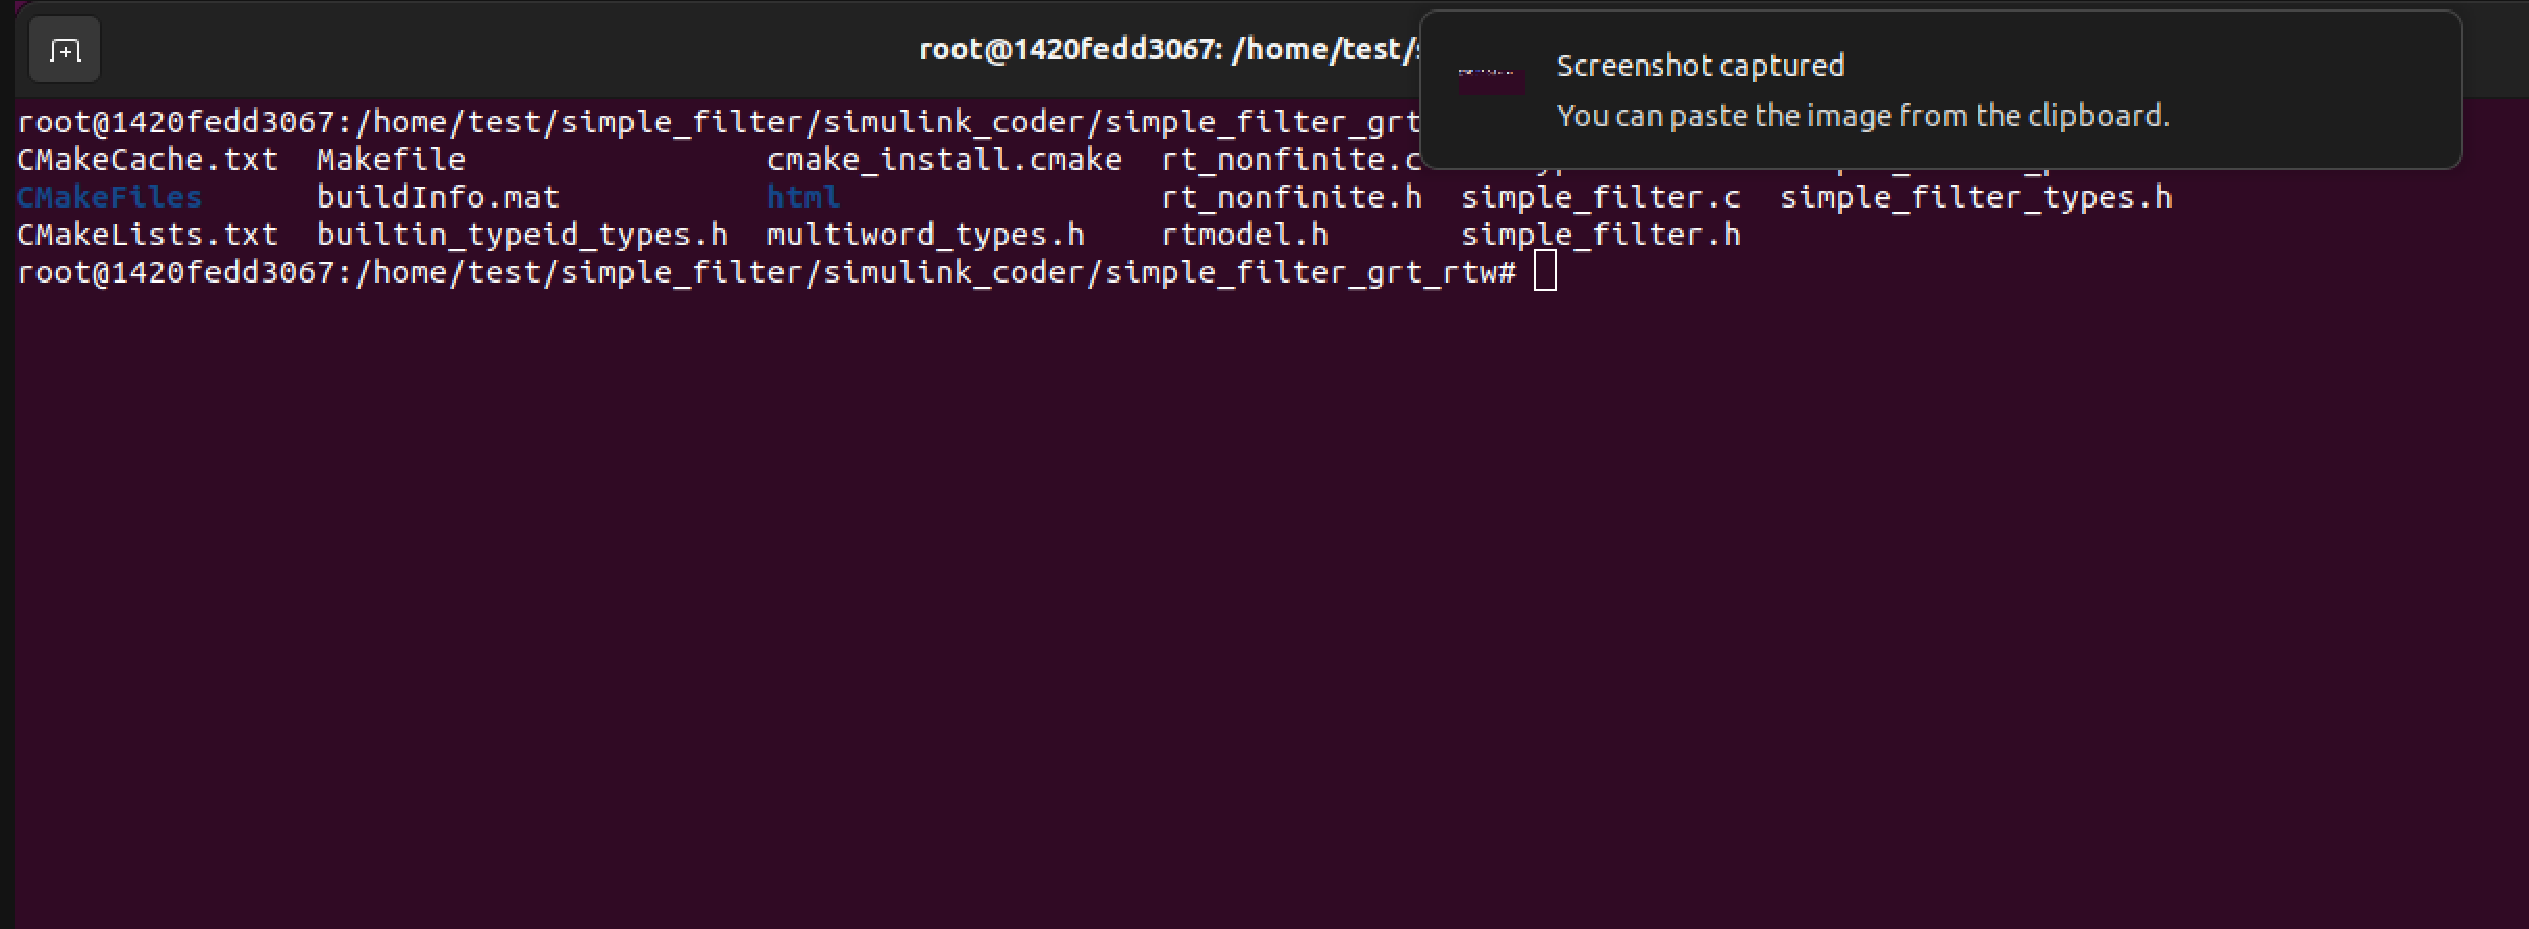
\includegraphics[width=0.8\textwidth]{fig/especifico_2/M2MT/paso_a_paso_mtmt/cmake_file.pdf}
    \caption{Make File}
    \label{fig:make_file}
\end{figure}


\begin{figure}[h!]
    \centering
    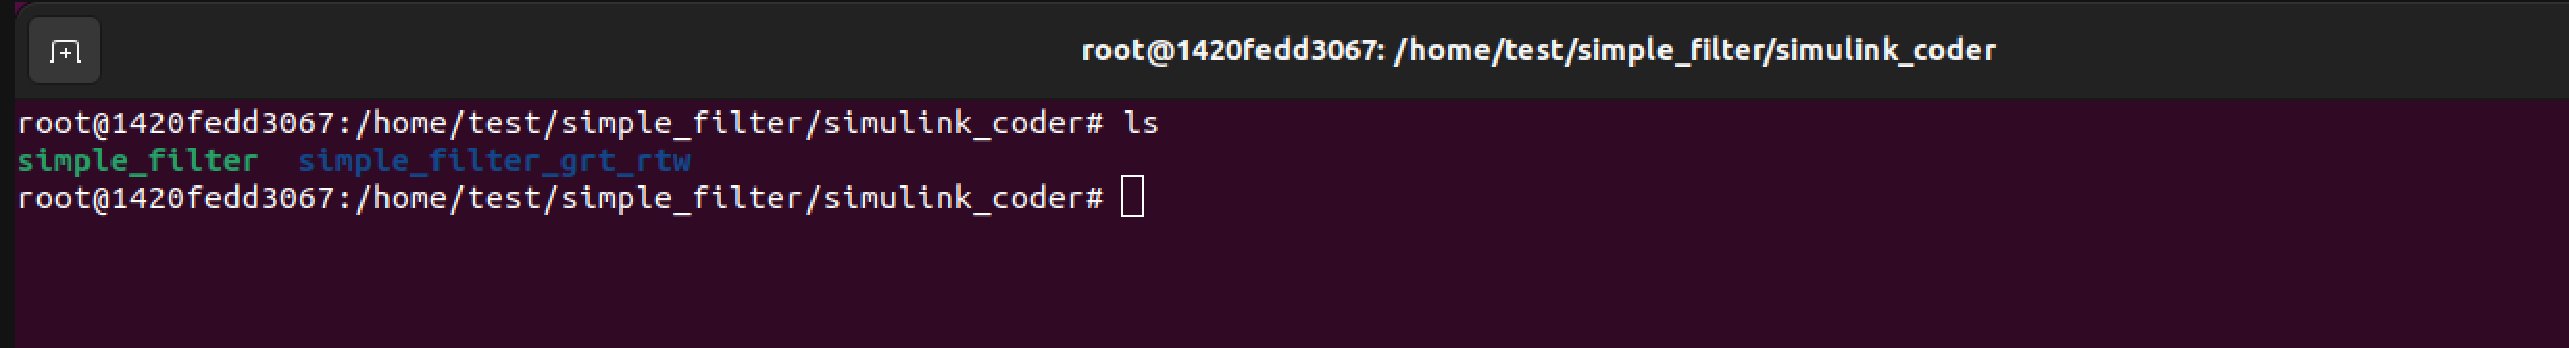
\includegraphics[width=0.8\textwidth]{fig/especifico_2/M2MT/paso_a_paso_mtmt/binario_compilado.pdf}
    \caption{Binario llamado simple\_filter}
    \label{fig:binario_compilado}
\end{figure}

Para la compilación del archivo binario se deberá hace uso del comando \ref{lst:build_cmake_file} por el cual se construirá el Makefile, tal y como se muestra en la Figura \ref{fig:make_file}, una vez generado el Makefile se ejecutó el comando (Make) el cual da como salida los binarios requeridos para la ejecución del programa. Los mismos se observan como se muestra en la Figura \ref{fig:binario_compilado}.

Una vez compilado el archivo binario, se puede continuar con el flujo que se presenta en el diagrama que se muestra en la Figura \ref{fig:diagrama_flujo_trabajo}, lo cual sería la implementación de los binarios en una imagen de yocto.
\newpage

\section{Flujo de Trabajo EmbedSynthGNC}

\begin{figure}[h!]
    \centering
    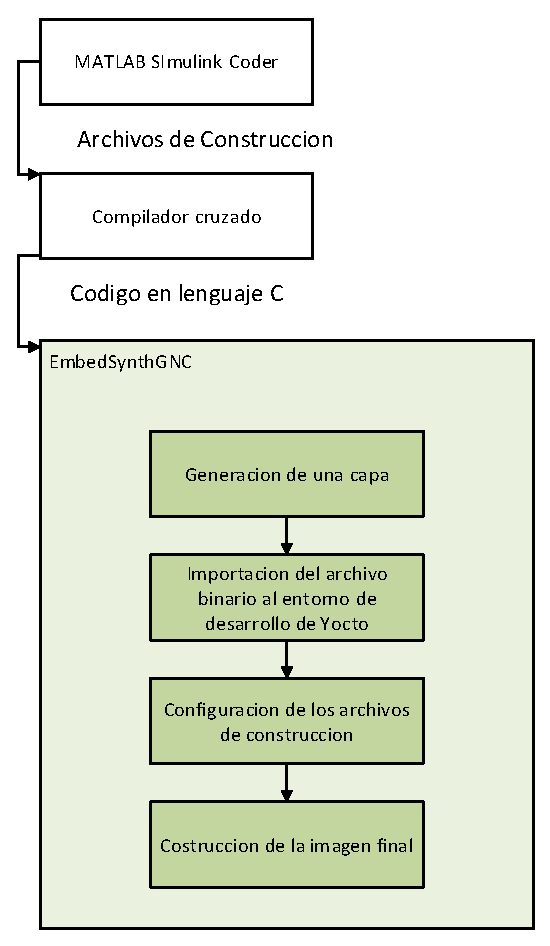
\includegraphics[width=0.8\textwidth]{fig/especifico_2/embedsynthgnc/diagrama_general_embedsynthgnc.pdf}
    \caption{Flujo de trabajo EmbedSynthGNC}
    \label{fig:diagrama_embed_synth_gnc}
\end{figure}

Como se pudo observar anteriormente se realizó la compilación cruzada de un caso de estudio, el mismo ahora se debe de implementar en un sistema operativo a la medida mediante el flujo de trabajo de Yocto Project, como se mencionó en \ref{subsec:yocto}, Yocto Project es un marco de trabajo utilizado para el desarrollo de sistemas embebidos especializado en la construcción de distribuciones de Linux a la medida, cabe destacar que el flujo de trabajo a seguir se explica brevemente en la Figura \ref{fig:diagrama_embed_synth_gnc}. 

En el desarrollo de esta sección se muestran los pasos que se siguieron para la generación de una imagen, la integración de una capa personalizada con el binario generado en \ref{subsec:compilacion_binario} y la implementación de la misma en la tarjeta de desarrollo seleccionada.

\subsection{Creación de una capa de yocto}

\begin{lstlisting}[language=bash, caption={"Print Working Directory",Linux}, label=lst:pwd]
    pwd
\end{lstlisting}

\begin{lstlisting}[language=bash, caption={Inicializar ambiente, Yocto}, label=lst:yocto_ambient_set]
    source oe-init-build-env build/
\end{lstlisting}

Para la generación de una capa de yocto primero debemos de estar seguros que nos encontramos en el directorio denominado POKY, esto lo podemos verificar por medio del uso del comando \ref{lst:pwd}, seguido de esto se debe de inicializar el entorno de desarrollo esto mediante el comando que se muestra en \ref{lst:yocto_ambient_set}, este se encarga de inicializar el entorno así también como todos los requerimientos necesarios para poder hacer uso de las variables de entorno con las cuales opera el marco de trabajo.

\begin{lstlisting}[language=bash, caption={Generar nueva capa, Yocto }, label=lst:yocto_new_layer]
    bitbake-layers create-layer <nombre-de-la-capa>
\end{lstlisting}

\begin{figure}[h!]
    \centering
    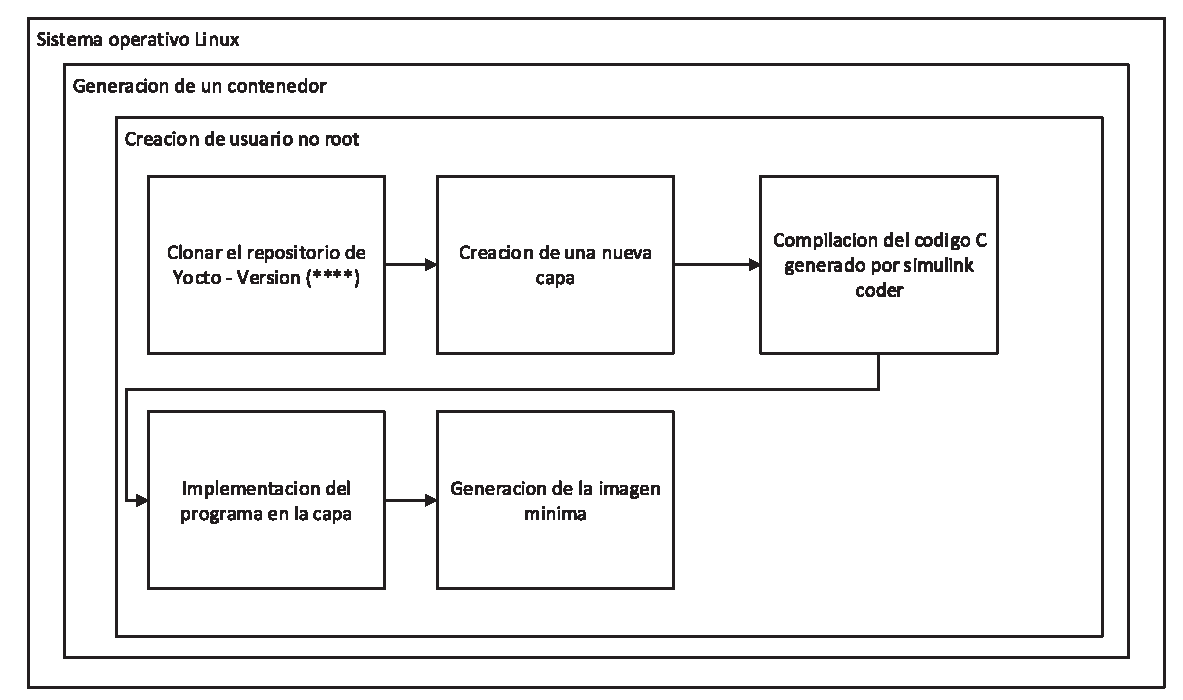
\includegraphics[width=0.8\textwidth]{fig/especifico_2/Flujo de trabajo de mi idea.pdf}
    \caption{Árbol de directorios de la capa}
    \label{fig:arbol_capa_custom_yocto}
\end{figure}

\begin{lstlisting}[language=bash, caption={Agregar nueva capa, Yocto }, label=lst:add_new_layer]
    bitbake-layers add-layer ../<nombre-de-la-capa>
\end{lstlisting}

Seguido de esto se debe de utilizar el comando que se muestra en \ref{lst:yocto_new_layer} el cual se encargara de generar el árbol de directorios que se puede observar en la Figura \ref{fig:arbol_capa_custom_yocto}. Una vez implementado este comando se debe de hacer uso del comando que se muestra en \ref{lst:add_new_layer} para poder agregar la capa al archivo denominado bblayers.conf el cual contiene todas las rutas de acceso a las capas requeridas para generar la imagen. Para este caso de estudio se debe de generar una capa con el nombre de (meta-embedsynthGNC).


\subsection{Caso de estudio 1 - Filtro Básico en ZedBoard}

En esta sección se integrará el caso de estudio generado en \ref{subsec:compilacion_binario}, a un sistema operativo a la medida por medio del marco de trabajo de Yocto Project.

\subsection{Integración del programa generado a la capa de Yocto}

Para la implementación del binario generado en \ref{subsec:compilacion_binario}, se deben de generar algunos directorios, esto con el objetivo de mantener un entorno de trabajo limpio y ordenado. Para contener todos los directorios que se deben de crear, se genera un directorio llamado (recipes-core) el cual dentro del mismo deberá de contener un directorio llamado (caso\_de\_estudio\_1) el cual se encargara de contener el archivo de configuración de la capa llamado (caso\_de\_estudio\_1.bb); este archivo se genera mediante el comando que se observa en \ref{lst:yocto_new_layer}, además de generar este archivo se debe de crear un directorio llamado "files" que será el encargado de contener el archivo binario compilado en \ref{subsec:compilacion_binario}.

\subsubsection{caso\_de\_estudio\_1.bb}

Como se mencionó anteriormente el archivo llamado sistema\_control.bb es el encargado de la configuración de la capa, el mismo contiene los comandos de instalación y la dirección en donde se encontrara el archivo binario en el sistema de archivos de la imagen del sistema embebido.

\begin{figure}[h!]
    \centering
    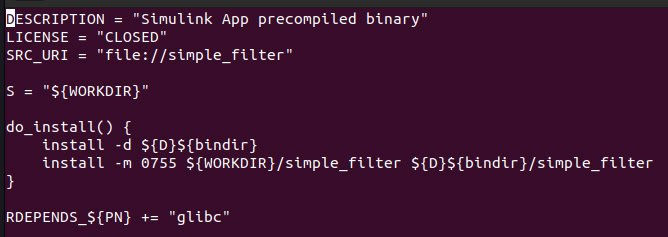
\includegraphics[width=0.8\textwidth]{fig/especifico_2/bbfilestructure.jpg}
    \caption{Estructura del archivo caso\_de\_estudio\_1.bb}
    \label{fig:estructura_archivo_bb}
\end{figure}

La estructura que debe de contener ese archivo para instalar binarios en el sistema son las que se pueden observar en la Figura \ref{fig:estructura_archivo_bb}.

\subsection{Generación de la imagen}\label{subsec:generacion_imagen_minima}

\begin{lstlisting}[language=bash, caption={Generar archivos de desarrollador, Yocto }, label=lst:yocto_developer_image]
    bitbake-layers add-layer ../<nombre-de-la-capa>
\end{lstlisting}

Antes de generar la imagen mínima se debe de tener en consideración ejecutar la línea de comando que se muestra en \ref{lst:yocto_developer_image}, esto con el fin de generar archivos de desarrollo en lugar de archivos de imagen en formato iso. Una vez generados estos cambios se debe de iniciar de nuevo el entorno por medio del comando \ref{lst:yocto_ambient_set}, seguido de esto se deberá de ejecutar el comando de "bitbake core-image-minimal" el cual se encarga de comenzar a generar la imagen mínima.

\begin{lstlisting}[language=bash, caption={Instalar la capa generada, Yocto }, label=lst:install_layer]
    IMAGE_INSTALL_APPEND+= caso\_de\_estudio\_1
\end{lstlisting}

Finalmente para la instalación de la capa dentro de la imagen se debe de editar el archivo de configuracion local llamado local.conf el cual se encuentra en la direccion build/conf/local.conf en el cual se debera de agregar la linea que se muestra en \ref{lst:install_layer} , esto con el fin de agregar la capa generada anteriormente al sistema de archivos de la imagen a generar.


\subsection{Implementación de la imagen mínima en la tarjeta de desarrollo Zedboard}

Para la implementación de la imagen mínima desarrollada en \ref{subsec:generacion_imagen_minima} en la tarjeta de desarrollo, se deben de desarrollar los siguientes pasos en la máquina Host, Primeramente se debe de formatear la tarjeta SD de al menos 4 GB, las particiones de la misma se tienen que observar de la siguiente forma:

\begin{itemize}
    \item raíz = 100 MB FAT 32
    \item sistema de archivos = 3.5 GB ext6(linux filesystem format)
\end{itemize} 

Seguido de esto se debe de ir a la ruta (ruta donde se encuentran los archivos de imagen de la zedboard), mientras que en la máquina host se debe de ir a la ruta seleccionada para almacenar los archivos temporalmente y se deben de copiar los archivos del contenedor a la máquina host mediante el comando que se muestra en \ref{lst:copy_from_container}, esto con el objetivo de poder enviar los archivos a la tarjeta SD más adelante.

\begin{lstlisting}[language=bash, caption={Copiar archivos root, Linux}, label=lst:copy_root]
    sudo cp boot.bin boot.scr 
    core-image-minimal-zedboard-zynq7.cpio.gz.u-boot
     u-boot.img uEnv.txt uImage zynq-zed.dtb /media/root
\end{lstlisting}

\begin{lstlisting}[language=bash, caption={Copiar sistema de archivos, Linux}, label=lst:copy_fs]
    sudo cp core-image-minimal-zedboard-zynq7.tar.gz /mnt/partition2
\end{lstlisting}

Para el sistema Root se deberán de copiar los archivos mediante el comando que se muestra en \ref{lst:copy_root}, por otro lado en la partición denominada FileSystem se debe de copiar el archvivo "core-image-minimal-zedboard-zynq7.tar.gz" mediante el uso del comando que se muestra en \ref{lst:copy_fs}.

\subsection{Conexión de la tarjeta de desarrollo con el computador host}

Como protocolo de comunicación se establece primeramente el protocolo UART, el cual como se mencionó en \ref{sec:protocolos_de_comunicacion} consiste en un protocolo de comunicación serie que permite la transmisión y recepción de datos de manera asíncrona entre dos dispositivos y en el caso de la tarjeta de desarrollo se conecta según se muestra en el diagrama de la Figura \ref{fig:puertos_zedboard}, mediante el uso del puerto marcado como "S" en el diagrama. Para poder leer la consola se hace uso de Minicom el cual se encarga de la emulación de terminal en Linux que permite la comunicación serie con dispositivos a través de puertos seriales.

\begin{figure}[h!]
    \centering
    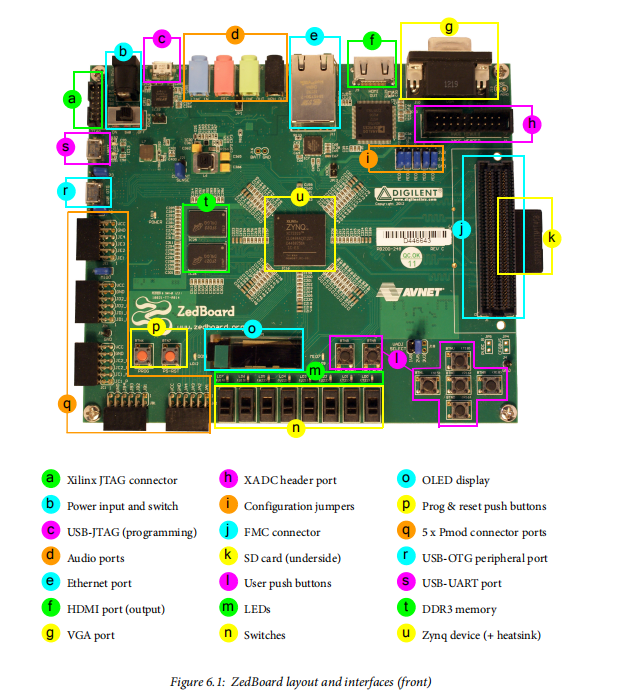
\includegraphics[width=0.8\textwidth]{fig/especifico_2/154140ZedBoard.png}
    \caption{Puertos tarjeta de desarrollo Zedboard}
    \label{fig:puertos_zedboard}
\end{figure}


Una vez que se estableció la conexión por medio de SSH el cual como se menciona en \ref{sec:protocolos_de_comunicacion}, consiste en protocolo de comunicación en red que permite el acceso remoto seguro a sistemas, proporcionando autenticación y encriptación de datos, ya que es mejor que UART para comunicaciones remotas porque proporciona autenticación y encriptación, garantizando la seguridad de los datos transmitidos, mientras que UART es un protocolo simple y sin mecanismos de seguridad, adecuado solo para comunicaciones locales y de corto alcance. 

El diagrama de este protocolo de comunicación se puede observar en \ref{fig:puertos_zedboard}, el cual se logra mediante la conexión al puerto denominado en el diagrama como e.


\subsection{Ejecución del caso de estudio y resultados}

Una vez implementada la imagen de Yocto en la tarjeta de desarrollo se puede ejecutar el caso de estudio. Para esto será necesario dirigirnos al directorio en el cual se instaló el archivo binario, el mismo se encuentra en la ruta usr-bin-simple\_filter. Una vez encontrado el archivo basta con ejecutarlo mediante el uso del nombre del mismo simple\_filter. Cuando el archivo se ejecuta genera dos archivos de salida llamados Raw\_signal.mat y Filtered\_signal.mat, mediante el uso del programa en Python desarrollado se pueden leer los archivos generados y crear gráficos a partir de los mismos. Los resultados se deben de transmitir al computador por medio del comando \ref{lst:copy_ssh}.

\begin{lstlisting}[language=bash, caption={Copiar archivo por protocolo SSH, Linux}, label=lst:copy_ssh]
    scp user@ip:/ruta/del/archivo/zedboard .
\end{lstlisting}

\begin{figure}[htbp]
    \centering
    \begin{subfigure}[b]{0.45\textwidth}
        \centering
        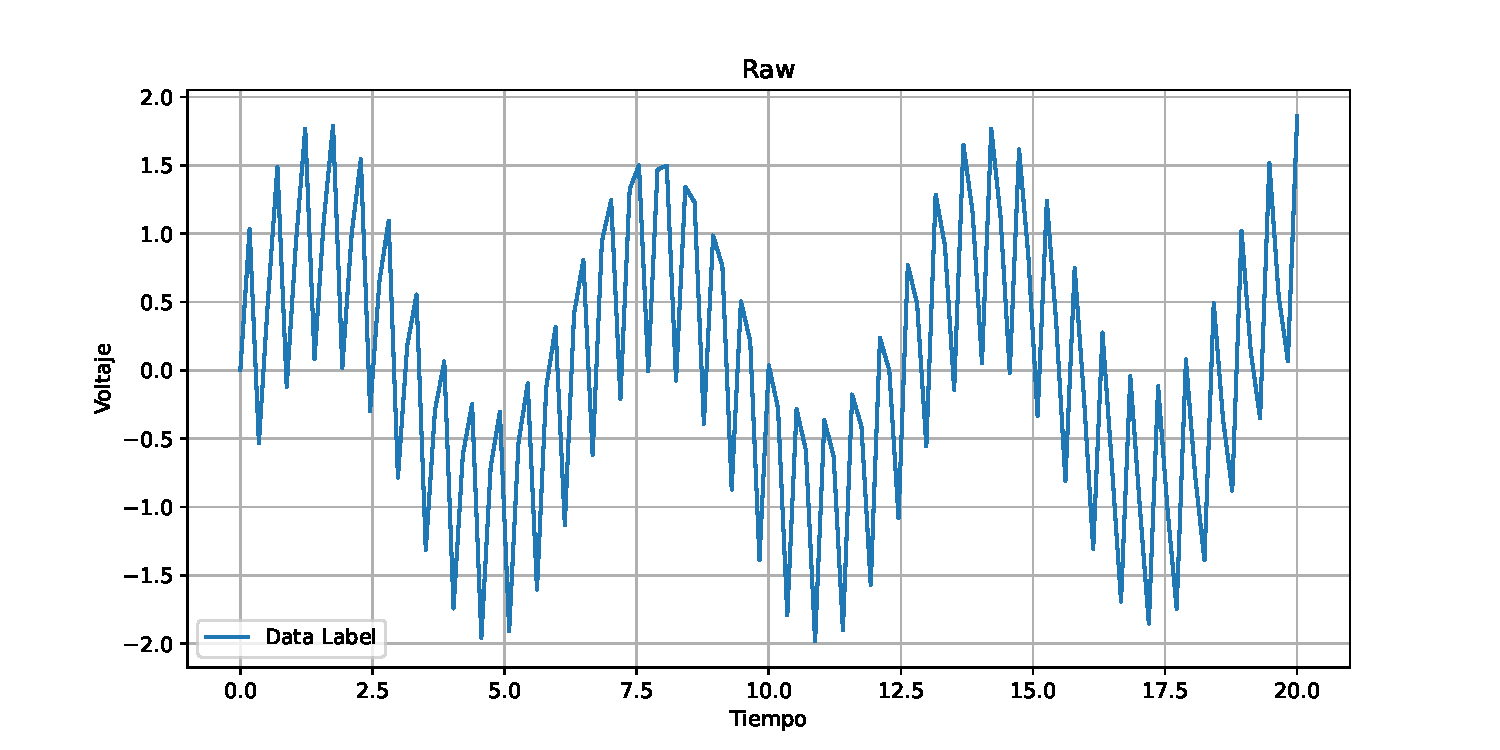
\includegraphics[width=\textwidth]{fig/especifico_2/raw.pdf}
        \caption{Ondas Moduladas}
        \label{fig:onda_modulada_zedboard}
    \end{subfigure}
    \hfill
    \begin{subfigure}[b]{0.45\textwidth}
        \centering
        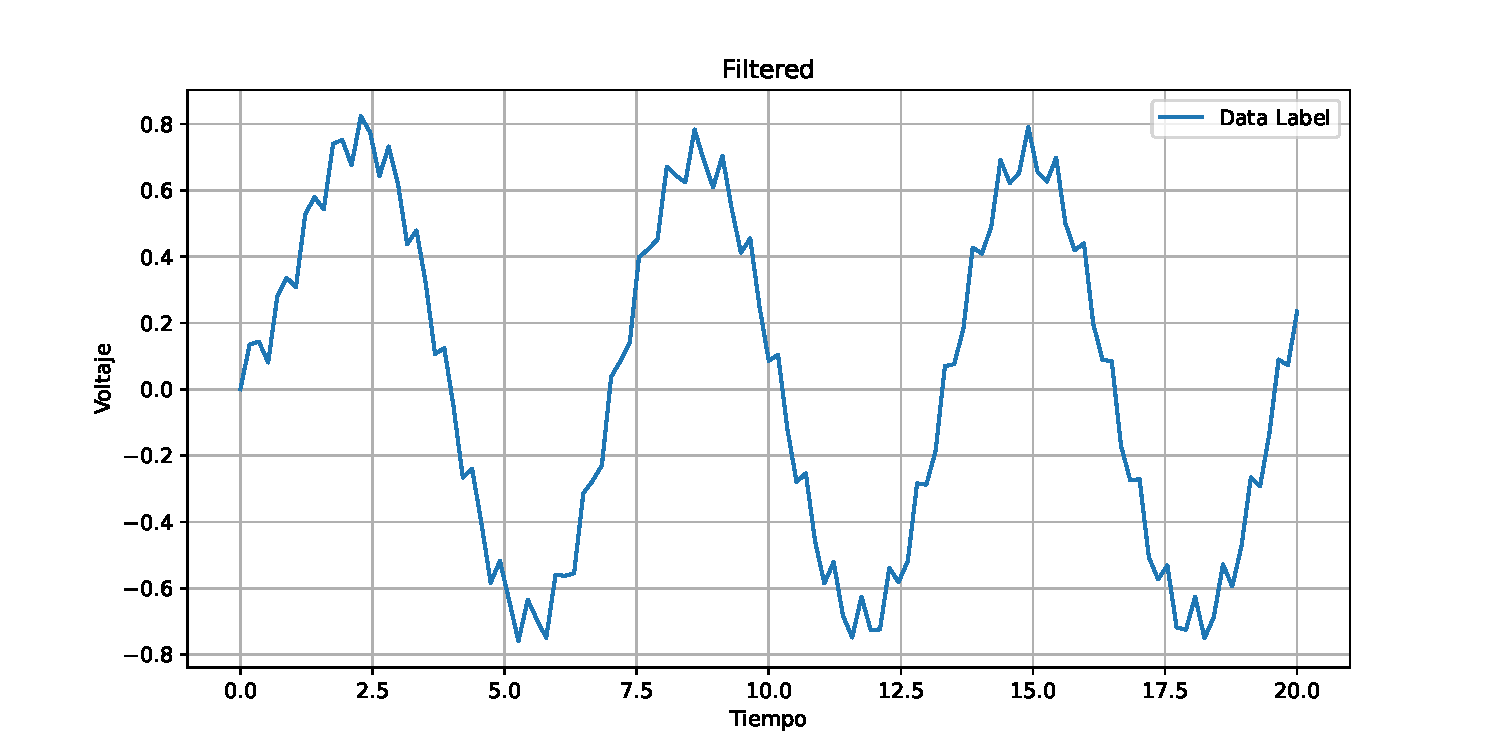
\includegraphics[width=\textwidth]{fig/especifico_2/Filtered.pdf}
        \caption{Onda resultante luego de la función de transferencia}
        \label{fig:onda_filtrada_zedboard}
    \end{subfigure}
    \caption{Salida resultante de la imagen generada mediante el flujo de trabajo}
    \label{fig:salida_resultante_diagrama_graficos_zedboard}
\end{figure}

\subsection{Comparación de resultados}

\begin{figure}[htbp]
    \centering
    \begin{subfigure}[b]{0.35\textwidth}
        \centering
        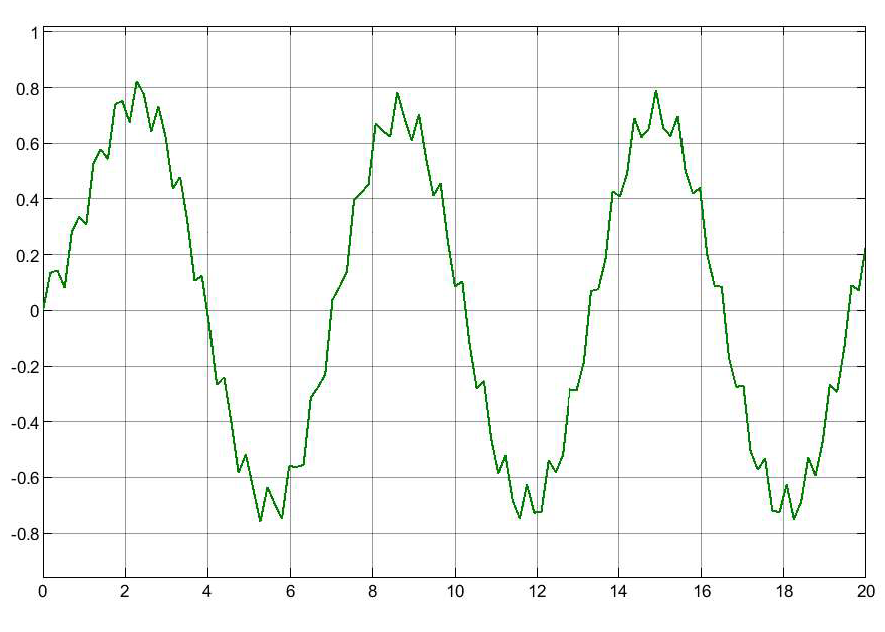
\includegraphics[width=\textwidth]{fig/especifico_2/onda_filtrada.pdf}
        \caption{Onda simulada resultante luego de la función de transferencia}
        \label{fig:onda_filtrada_simulada_matlab}
    \end{subfigure}
    \hfill
    \begin{subfigure}[b]{0.45\textwidth}
        \centering
        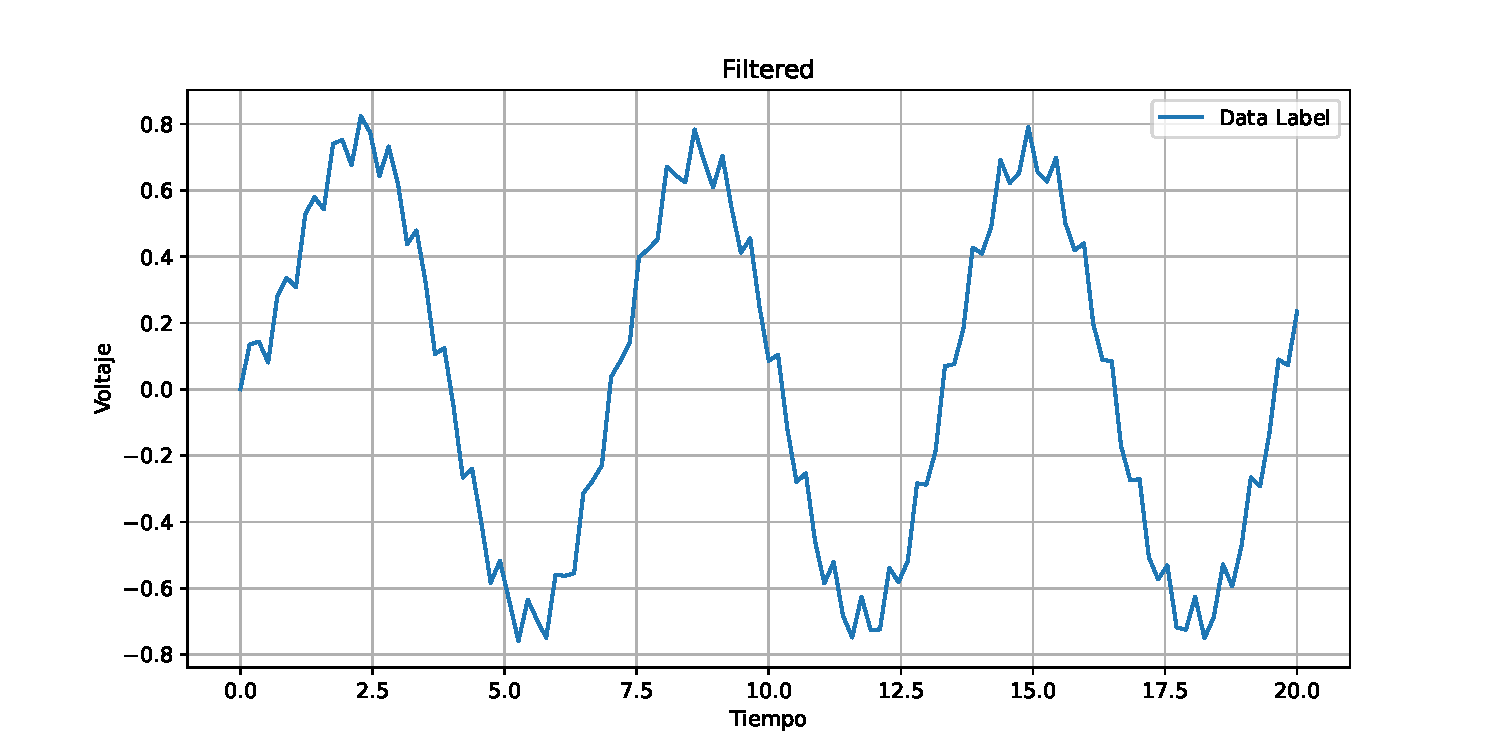
\includegraphics[width=\textwidth]{fig/especifico_2/Filtered.pdf}
        \caption{Onda experimental resultante luego de la función de transferencia}
        \label{fig:onda_filtrada_experimental_zedboard}
    \end{subfigure}
    \caption{Comparación de la salida resultante simulada (izquierda) y experimental (derecha)}
    \label{fig:comparacion_salida_resultante}
\end{figure}

Como se pudo observar en la Figura \ref{fig:comparacion_salida_resultante}, a la izquierda se puede observar la gráfica proveniente de la simulación del sistema, por otro lado en la derecha se puede observar la gráfica proveniente de la ejecución del sistema en la tarjeta de desarrollo, estas mediciones corresponden a las señales resultantes luego de la etapa de filtrado del caso de estudio desarrollado en esta sección. 

Para un mejor análisis de resultados se utilizó el código de Python que se muestra en \ref{apx:comparacion_de_sennales_programa}, el cual se encarga de tomar tanto el archivo de salida de la simulación como el archivo de salida del caso experimental y compararlas, esto con el objetivo de poder medir el error promedio absoluto, el error cuadrático medio y la raíz cuadrada del mismo, esto con el objetivo de poder cuantificar las diferencias entre la señal de salida simulada y la experimental.

Para este caso de estudio se obtuvieron los siguientes resultados:

\begin{itemize}
    \item Error Promedio Absoluto = $1.930 \times 10^{-18}$ [V]
    \item Error Cuadrático Medio = $2.14 \times 10^{-34}$ $[V^{2}]$
    \item Raíz del Error Cuadrático Medio = $1.46 \times 10{-17}$ [V]
\end{itemize}

Los valores de error obtenidos son bajos, lo cual nos indica un alto nivel de correspondencia entre la señal simulada y la señal experimental. Por un lado tenemos el error promedio absoluto, el cual represente la diferencia promedio entre la simulación y el experimento, al ser esta métrica representada por un valor de $1.930 \times 10^{-18}$ V sugiere que las diferencias entre ambas señales son despreciables. Por otro lado, tenemos el error cuadrático medio, este es asociado con un valor de $2.14 \times 10^{-34}$ $V^{2}$, lo que indica que las desviaciones en las mediciones son mínimas y puntuales. Finalmente la raíz del error cuadrático medio, la cual es representada por el valor de $1.46 \times 10{-17}$ V representa la magnitud promedio de las diferencias cuadráticas. La cercanía a cero que otorga este valor refuerza la alta precisión del modelo en relación con la señal experimental.

Al tener valores tan bajos en las métricas encargadas de medir el error de los modelos se puede respaldar que el proceso experimental es acorde a los resultados de simulación, cumpliendo con los requisitos de exactitud de forma notable.

\section{Reflexión final}

Los resultados de error obtenidos son altamente satisfactorios, lo cual respalda la implementación del caso de estudio realizada a lo largo de este capítulo. Estos valores indican una correspondencia prácticamente perfecta entre la simulación y el proceso experimental. La alta precisión alcanzada no solo válida el modelo desarrollado, sino que también resalta la consistencia y fiabilidad del proceso experimental. Es por esto que se aprueba el marco de trabajo realizado y se continúa con la investigación del mismo.
